\documentclass[12px]{article}

\title{Dispense Di Geometria I}
\date{2024-06-06}
\author{Federico De Sisti}

\usepackage{amsmath}
\usepackage{amsthm}
\usepackage{mdframed}
\usepackage{amssymb}
\usepackage{nicematrix}
\usepackage{amsfonts}
\usepackage{tcolorbox}
\tcbuselibrary{theorems}
\usepackage{xcolor}
\usepackage{cancel}

\newtheoremstyle{break}
  {1px}{1px}%
  {\itshape}{}%
  {\bfseries}{}%
  {\newline}{}%
\theoremstyle{break}
\newtheorem{theo}{Teorema}
\theoremstyle{break}
\newtheorem{lemma}{Lemma}
\theoremstyle{break}
\newtheorem{defin}{Definizione}
\theoremstyle{break}
\newtheorem{propo}{Proposizione}
\theoremstyle{break}
\newtheorem*{dimo}{Dimostrazione}
\theoremstyle{break}
\newtheorem*{es}{Esempio}

\newenvironment{dimo}
  {\begin{dimostrazione}}
  {\hfill\square\end{dimostrazione}}

\newenvironment{teo}
{\begin{mdframed}[linecolor=red, backgroundcolor=red!10]\begin{theo}}
  {\end{theo}\end{mdframed}}

\newenvironment{nome}
{\begin{mdframed}[linecolor=green, backgroundcolor=green!10]\begin{nomen}}
  {\end{nomen}\end{mdframed}}

\newenvironment{prop}
{\begin{mdframed}[linecolor=red, backgroundcolor=red!10]\begin{propo}}
  {\end{propo}\end{mdframed}}

\newenvironment{defi}
{\begin{mdframed}[linecolor=orange, backgroundcolor=orange!10]\begin{defin}}
  {\end{defin}\end{mdframed}}

\newenvironment{lemm}
{\begin{mdframed}[linecolor=red, backgroundcolor=red!10]\begin{lemma}}
  {\end{lemma}\end{mdframed}}

\newcommand{\icol}[1]{% inline column vector
  \left(\begin{smallmatrix}#1\end{smallmatrix}\right)%
}

\newcommand{\irow}[1]{% inline row vector
  \begin{smallmatrix}(#1)\end{smallmatrix}%
}

\newcommand{\matrice}[1]{% inline column vector
  \begin{pmatrix}#1\end{pmatrix}%
}

\newcommand{\C}{\mathbb{C}}
\newcommand{\K}{\mathbb{K}}
\newcommand{\R}{\mathbb{R}}


\begin{document}
	\maketitle
	\newpage
	\section{Geometria Affine}
	\subsection{Spazi Affini}
	\begin{defi}[Spazio affine]
		Sia $V$ uno spazio vettoriale su $\K$. Uno spazio affine su $V$ è un insieme non vuoto $\A$ i cui elementi si dicono punti di $A$ tale che sia data un'applicazione
		\[
			A\times A \rightarrow V \ \ \ [1.1]
		.\] 
		che associa ad ogni $(P,Q)\in A\times A$ un vettore di  $V$, denotato con $ \overrightarrow{PQ}$ e chiamato vettore di punto iniziale $P$ e punto  $Q$, in modo che i seguenti due assiomi siano soddisfatti.
		\begin{itemize}
			\item[-] Per ogni punto $P\in \A$ e per ogni vettore $v\in V$ esiste un unico punto $Q\in \A$ tale che
				\[
				 \overrightarrow{PQ} = v
				.\]  
			\item[-] Per ogni terna $P,Q,R$ di punti di $\A$ è soddisfatta la seguente identità
				\[
				 \overrightarrow{PQ}+\overrightarrow{QR}=\overrightarrow{PR}
				.\] 
		\end{itemize}
				L'applicazione $[7.1]$ definisce una struttura di spazio affine sull'insieme  $\A$
	\end{defi}
	\begin{defi}[Rifermineto affine]
		Siano $V$ su $\K$-spazio vettoriale e $\A$ uno spazio affine su $V$. Un sistema di coordinate affine (ovvero un riferimento affine) nello spazio $\A$ è assegnato una volta fissati un punto $O\in A$ e una base $ \{e_1,\ldots,e_n\}$ di $V$; esso viene denotato con $Oe_1,\ldots,e_n$
	\end{defi}
	\begin{defi}[Coordinate affini]
		Per ogni punto $P\in A$ si ha $ \overrightarrow{OP} = a_1e_1+\ldots+a_ne_n$ per opportuni $a_1,\ldots, a_n\in \K$.\\
		Gli scalari $a_1,\ldots,a_n$ si dicono coordinate affini. Il punto $O$ si dice origine del sistema di coordinate $(0,\ldots,0)$
	\end{defi}
	\begin{defi}[Giacitura]
		La giacitura di uno spazio affine è lo spazio vettoriale sul quale lo spazio affine è definito
	\end{defi}
	\newpage
	\begin{prop}
		1) Un sottospazio affine è individuato dalla sua giacitura e da uno qualsiasi dei suoi punti\\
		2) Sia $S$ un sottospazio affine di $\A$ avente giacitura $W$, Associando ad ogni coppia di punti $P,Q$ di $S$ il vettore $\overrightarrow{PQ}$ si definisce su $S$ una struttura di spazio affine su $W$
	\end{prop}
	\begin{dimo}
		1) Sia  $S$ il sottospazio affine di $\A$ passante per $Q$ ed avente giacitura $W$. Sia $M\in S$ e sia $T$ il sottospazio affine passante per $M$ ed avente giacitura $W$. Se $P\in S$ allora si ha
		\[
		 \overrightarrow{MP}=\overrightarrow{MQ}+\overrightarrow{QP} = - \overrightarrow{QM} + \overrightarrow{QP}
		.\] 
		che è un vettore di $W$ perché entrambe gli addendi vi appartengono, quindi $P\in T$.\\
		Se viceversa $P\in T,$ allora
		\[
		\overrightarrow{QP} = \overrightarrow{QM} + \overrightarrow{MP} = - \overrightarrow{MQ} + \overrightarrow{MQ}\in W
		.\] 
		e quindi $P\in S$. In conclusione $S=T$\\
		2) Se $ P,Q\in S$ allora $\overrightarrow{PQ}\in W$ perché, per la (1), $S$ coincide con il sottospazio affine passante per $P$ e parallelo a $W$. Otteniamo quindi un'applicazione\ \ \  \ 
		\begin{aligend}
			\text{   \ \ \ \ \  }&S\times S \rightarrow W\\
			\text{   \ \ \ \   }&(P,Q) \rightarrow \overrightarrow{PQ}
		\end{aligend}\\
		la quale soddisfa le proprietà dell'applicazione che definisce la struttura di spazio affine, perché sono verificate in $\A$
	\end{dimo}
	\textbf{Osservazioni}\\
	1) Possiamo quindi definire sottospazi affini di $(A,V)$ come i sottospazi del tipo \[
		p + W \ \ \ \ W\subseteq V \ \ \text{sottospazio vettoriale}
	.\] 
	Ricordiamo anche che $p + W = q + W \Leftrightarrow \overrightarrow{PQ}\in W$ \ \\[10px]2) Se $\Sigma_1 = p_1 + W_1, \ \ \Simga_2 = p_2 + W_2$ sono sottospazi affini , la loro intersezione, se non vuota, è un sottospazio affine. Infatti $p\in\Sigma_1\cap\Sigma_2$ 
	\[
	\Sigma_1\cap\Sigma_2=p + W_1\cap W_2
	.\] 
	\begin{lemm}
		$\emptyset\neq S\subset A \ \ \ \ p,q\in S$\\
		$H_p = \{\overrightarrow{px}\ \ |\ \ x\in S\} \ H_q =\{ \overrightarrow{qy}\ \ |\ \ y\in S\}$\\
		Allora $<H_p> = <H_q>$ e $p + <H_p> = q + <H_q>$ \\(sottospazio generato da $S$)
	\end{lemm}
	\begin{dimo}
		\begin{aliged}
		&v_0 = \overrightarrow{pq} \ \ v_0\in H_p \ \ -v_0 = \overrightarrow{qp}\in H_q \\
		&H_p\ni \overrightarrow{px} = \overrightarrow{pq} + \overrightarrow{qx} = v_0 + \overrightarrow{qx}\in <H_q>\\
		& H_p \ \subseteq \ <H_q>\ \  \Rightarrow\ \ \ <H_p>\ \subseteq \ <H_q>\\
		&H_q\ni \overrightarrow{qy} = \overrightarrow{qp} + \overrightarrow{py}\in <H_q>\ \Rightarrow  \ <H_q>\ \subseteq \ <H_p>
		\end{aliged} \\
		Quindi \begin{aligend}
			&<H_p> = <H_q> \\
			&\overrightarrow{pq}\in<H_p> = <H_q>\\
			&p + <H_p> = q + <H_q>
		\end{aligend}
	\end{dimo}
	\begin{nome}
		$\Sigma_1,\Sigma_2$ sottospazi affini \[
			\Sigma_1 \vee \Sigma_2 := \text{sottospazio generato da } \Sigma_1\cup\Sigma_2
		.\] 
	\end{nome}
	\begin{lemm}
		Siano $\Sigma_i = p_i + W_i, \ \ \ i = 1,2$ sottospazi affini. Allora\\
		(a) $\Sigma_1\cap\Sigma_2\neq\emptyset \Leftrightarrow \overrightarrow{p_1p_2}\in W_1+W_2\\$
		(b) $\Sigma_1\vee\Sigma_2 = p_1 + (W_1 + W_2 + <\overrightarrow{p_1p_2}>)$
	\end{lemm}
	\begin{dimo}
		(a) $p_0\in\Sigma_1\cap\Sigma_2$ allora
		\begin{aligend}
			&\Sigma_1 = p_0 + W_1 \ \ \Simga_2 = p_0+W_2\\
			&\exists w_i\in W_i, \ \ i = 1,2 \ \ \text{ t.c }\\
			&p_1 = p_0 + W_1, p_2 = p_0 + W_2\\
			&\overrightarrow{p_1p_2} = w_2-w_1\in W_1 + W_2\\
		\end{aligend}
		Viceversa, se $\overrightarrow{p_1p_2} = w_1 + w_2, w_1\in W_1, w_2\in W_2 $\\
		\begin{aligned}
			&p_2 = p_1 + \overrightarrow{p_1p_2} = p_1 + w_1 + w_2\\
			&p_2 - w_2 = p_1 + w_1 \in \Sigma_1\cap\Sigma_2
		\end{aligned}
		(2) Dato $x\in\Sigma_1\cup\Sigma_2$, risulta \\
		$\overrightarrow{p_1x}\in W_1$ se $x\in\Sigma_1$ \\ 
		oppure
		\[
		\overrightarrow{p_1x}\in\overrightarrow{p_1p_2}+ W_2 \ \ (\overrightarrow{p_1x} = \overrightarrow{p_1p_2} + \overrightarrow{p_2x})
		.\] 
		Dunque la giacitura di $\Sigma_1\vee\Sigma_2$ è \[
		W_1 + W_2 + <\overrightarrow{p_1p_2}>
		.\] 
	\end{dimo}
	\newpage
	\subsection{Posizioni Reciproche di sottospazi affini}
	\begin{defi}
		Siano $\Sigma_1,\Sigma_2$ sottospazi affini di $(A,V)$ di giacitura rispettivamente $W_1,W_2$ Diciamo che \\
		1) $\Sigma_1,\Sigma_2$ sono \textbf{incidenti}, se \Sigma_1\cap\Sigma_2\neq\emptyset\\
		2) \ $\Sigma_1,\Sigma_2$ sono \textbf{paralleli} se $W_1\subseteq W_2$ o $W_2\subseteq W_1$\\
		3) $\Sigma_1,\Sigma_2$ sono \textbf{sghembi} se $\Sigma_1\cap\Sigma_2 = \emptyset$ e $W_1\cap W_2 = \{0\}$
	\end{defi}
	\textbf{Osservazione} \\
	Queste posizioni non sono mutuamente esclusive e non costituiscono tutte le possibilità\\
\begin{prop}[Fromula Grassmann per spazi affini]
	Siano $\Sigma_1, \Sigma_2 $ sottospazi affini di $A$, Allora 
	\[
	dim(\Sigma_1 \vee \Sigma_2) \leq dim\Sigma_1 + dim\Sigma_2 - dim(\Sigma_1\cap\Sigma_2)
	.\] 
	e vale l'uguaglianza se $\Sigma_1, \Sigma_2$ sono incidenti o sghembi\\
	si usa la notazione $dim(\emptyset) = -1$
\end{prop}
\begin{dimo}
	- Supponiamo $\Sigma_1,\Sigma_2$ incidenti, allora esiste
\begin{gather*}
	p_0 \in\Sigma_1\cap\Sigma_2 \\
	\Sigma_1 = p_0 + W_1, \Sigma_2 = p_0 + W_2\\
	\Sigma_1\cap\Sigma_2 = p_0 + W_1\cap W_2, \Sigma_1\vee\Sigma_2 = p_0 + W_1 + W_2
\end{gather*}
	dunque vale l'uguaglianza per Grassman vettoriale\\
	- Sia ora $\Sigma_1\cap\Sigma_2 = \emptyset$ allora $\Sigma_i = p_i + W_i$ ~ $i = 1, 2$\\
	risulta $\overrightarrow{p_1p_2}\notin W_1 + W_2$ (per lemma)\\
	\begin{gather*}
		dim(\Sigma_1\vee\Sigma_2) = dim(W_1 + W_2 + <\overrightarrow{p_1p_2}) = dim(W_1+W_2) + 1\leq \\ \leq dim(W_1) + dim(W_2) - (-1) = dim(W_1) + dim(W_2) + dim(\Sigma_1\cap\Sigma_2)
	\end{gather*}
	e vale l'uguaglianza se e solo se $dim(W_1) + dim(W_2) = dim(W_1 + W_2)$ ovvero $W_1\cap W_2 = {0}$ ovvero se $\Sigma_1, \Sigma_2$ sono sghembi $\hfill\square$	
\end{dimo}
\newpage
\begin{prop}
	siano $\Sigma_1, \Sigma_2$ sottospazi affini di $\mathbb{A}^n(\mathbb{K})$ definiti dai sistemi lineari \[
	A_iX = b_i \ i = 1,2
	.\]
	Allora:\\
	(a) $\Sigma_1, \Sigma_2$ sono incidenti se e solo se \[
		rk\begin{pNiceArray}{c|c}
			A_1 & b_1\\
			\hline
			A_2 & b_2 \\
			\end{pNiceArray} = rk \begin{pNiceArray}{c}
				A_1 \\
				\hline
				A_2
			\end{pNiceArray}
	.\] 
	detto r tale rango, $dim(\Sigma_1\cap\Sigma_2) = n-r$\\
	(b) $\Sigma_1, \Sigma_2$ sono sghembi se e solo se \[
		rk\begin{pNiceArray}{c|c}
			A_1 & b_1\\
			\hline
			A_2 & b_2 \\
			\end{pNiceArray} \geq rk \begin{pNiceArray}{c}
				A_1 \\
				\hline
				A_2
			\end{pNiceArray} = n
	.\] 
	(c) Se\[
		rk\begin{pNiceArray}{c|c}
			A_1 & b_1\\
			\hline
			A_2 & b_2 \\
			\end{pNiceArray} \geq rk \begin{pNiceArray}{c}
				A_1 \\
				\hline
				A_2
			\end{pNiceArray} = r < n
	.\] 
	allora $\Sigma_1$ (rispetto a $\Sigma_2$) contiene un sottospazio affine di dimensione $n-r$ parallelo a $\Sigma_2$ (rispetto a $\Sigma_1$)
\end{prop}
\begin{dimo}
	(a) $\Sigma_1 \cap\Sigma_2 \neq \emptyset \Leftrightarrow$ il  sistema è compatibile quindi tutto segue da Rochè-Capelli\\[10px]
	(b) la disuguaglianza tra i ranghi dice che $\Sigma_1\cap\Sigma_2 = \emptyset$;\\ il fatto che $rk \begin{pNiceArray}{c}
		A_1 \\
		\hline
		A_2
	\end{pNiceArray} = n$ implica che $W_1\cap W_2 = {0}$\\
(c) Di nuovo la disuguaglianza dei  ranghi implica $\Sigma_1\cap\Sigma_2 = \emptyset$;\\
Se ora $W_1\cap W_2 = W$ allora $dim(W_1\cap W_2) = n - r$\\
Scelto $p_1 \in \Sigma_1$ risulta\\
$p_1 + W \subset\Sigma_1$ \ ($W_1 \cap W_2 = W$ sottospazio di $W_1$)\\
e $W \subset W_2 \Rightarrow p_1 + W$ è parallelo a $\Sigma_2$ e $dim(p_1 + W) = dim(W) = n - r \hfill\square$
\end{dimo}
\begin{es}
	$\mathbb{A} \ \pi_1,\pi_2$ piani distinti\\
	$A_1,A_2$ vettori riga $(A_1 = (a_{11} \ a_{12} \ a_{13})\\
	C = \begin{pNiceArray}{c c}
		A_1 & b_1\\
		A_2 & b_2
	\end{pNiceArray} \in M_{2,4}(\mathbb{R})$\\
	piani distinti $\Rightarrow \ rk(C) = 2$\\
	$rg \begin{pNiceArray}{c}
		A_1 \\
		\hline
		A_2 \\
	\end{pNiceArray} = 2 \ \Rightarrow \pi_1\cap\pi_2$ è una retta\\
	$rg \begin{pNiceArray}{c}
		A_1 \\
		\hline
		A_2 \\
	\end{pNiceArray} = 1 \ \Rightarrow \pi_1\cap\pi_2 = \emptyset$ piani paralleli poiché $W_1 = W_2$\\
\end{es}
\newpage
$ \mathbb{A}^4, \pi_1\pi_2$ piani distinti tali che $rk(A_i|b_i) = 2$ \\
\[
C = \begin{pNiceArray}{c|c}
	A_1 & b_1 \\
	\hline
	A_2 & b_2 \\
\end{pNiceArray} \in M_{4\times5} \ \ rk(C)\leq 4
.\]
\[
\begin{tabular}{|c|c|c|}
	\hline
	rk \icol{A_1 \\ \hline  A_2} & rk(C) & \pi_1\cap \pi_2 \\ 
	\hline
	4 & 4 & \{p\} \\
	3 & 4 & \emptyset \text{ e } W_1, W_2 \text{ hanno una direzione in comune} \\
	3 & 3 & r \\
	2 & 3 & \emptyset\\
	\hline
\end{tabular}
\]
\subsection{Applicazioni affini}
$V, V'$ spazi vettoriali su $\mathbb{K}, (A,V,+), (A',V',+)$ spazi affini\\
\begin{defi}
	$f:A\rightarrow A'$ è un'applicazione affine se esiste un'applicazione lineare $\phi :V\rightarrow V'$ tale che:  \[
	f(p + v) = f(p) + \phi (v) \ \ \ \forall p\in A, \forall v\in V
	.\]
	\left( ovvero \  \ \ 
		\begin{aligned}
		& f(Q) = f(P) + \phi(\overrightarrow{PQ}) \ \ \forall P, Q\in A \\ 
		& \overrightarrow{f(P)f(Q)} = \phi(\overrightarrow{PQ})\ \ \ \ \   \forall P,Q\in A \\ 
	\end{aligned}
\right)
\end{defi}
\textbf{Nomenclatura}\\
Se $f$ è biunivoca, $f$ è detto isomorfismo affine\\
Un isomorfismo affine $A\rightarrow A$ è detto affinità.\\
\textbf{Osservazione}\\
vedremo che le affinità formano un gruppo rispetto alla composizione di applicazione che denoteremo come $\text{Aff}(A)$\\
\textbf{Esempio}\\
	$Ov_1...v_n$ rifermento affine in A\\
	\[
		f: \mathbb{A} \rightarrow \mathbb{A}^n \ \ f(p) = \begin{pNiceArray}{c}
			x_1\\
			.\\.\\
			x_n
		\end{pNiceArray} \ \ \  e \ \ \ \overrightarrow{OP} = \sum^n_{i=1}x_i v_i
	.\]
	Dico che f è un isomorfismo affine con associato isomorfismo lineare \\ $ \varphi ( \sum^n_{i=1}x_i v_0) = \begin{pNiceArray}{c}
		x_1 \\ . \\ . \\ x_n \\	
	\end{pNiceArray}$\\
	Verifichiamo che $\overrightarrow{f(P)f(Q)} = \varphi (\overrightarrow{PQ})\\
	\overrightarrow{OQ} = \sum^n_{i=1}y_iv_i \ \ \ f(Q) = \begin{pNiceArray}{c}
		y_1\\ . \\ . \\ y_n \\
	\end{pNiceArray}
	\overrightarrow{f(P)f(Q)} = \icol{y_1\\.\\.\\.\\y_n} - \icol{x_1\\.\\.\\.\\ x_n} = \icol{y_1 - x_1\\.\\.\\.\\y_n - x_n} =  \varphi ( \sum^n_{i=1}(y_i - x_i)v_i) = \varphi (\overrightarrow{OQ} - \overrightarrow{OP}) =  \varphi (\overrightarrow{PQ})$\\[10px]
\textbf{3 Esempi di affinità}\\
I traslazioni\\
Fissato $v\in V$ definiamo \\
$t_v:A\rightarrow A, \ \ t_v(P) = p + v$
Dico che $t_v$ è un'affinità con associato isomorfismo $Id_V$ dato che:\\
$t_V(p + w) = (p + w) + v = p + (w + v) = p + (v + w) = (p + v) + w =\\ = t_V(p) + w = t_V(p) +  \varphi (w) \leftarrow Id_V$ \\
la biunicità segue dagli assiomi per A \\[10px]
II Simmetria rispetto ad un punto\\
$\sigma_C(p) = C - \overrightarrow{CP}\\
$ Dico che $\sigma_C$ è un'affinità con parte lineare $ \varphi = -Id$\\
$\sigma_C(p + v) = c - \overrightarrow{CQ} \ \ Q = p + v \ \ v = \overrightarrow{PQ} \\
\sigma_C(p) + \phi(v) = c - \overrightarrow{CP} - v = c - \overrightarrow{CP} - \overrightarrow{PQ} = c - \overrightarrow{CQ}$ \\
III Otetia di centro O e fattore $\gamma\in\matbb{R}\backslash \{ 0 \} $ \\ 
\[
	\omega_{O,\gamma}(p) = O + \gamma \overrightarrow{OP}
.\] 
è un'affinità con parte lineare $\phi = \gamma Id_V$\\
$\omega_{O,\gamma}(p + v) = O + \gamma \overrightarrow{OQ} = O + \gamma( \overrightarrow{OP} + \overrightarrow{PQ}) = (O + \gamma \overrightarrow{OP}) + \gamma \overrightarrow{PQ} = \omega_{O,\gamma}(p) = \varphi(v)$

\begin{lemm}
	Fissato $O\in \mathbb{A} $, per ogni $O'\in \mathbb{A} $ e per ogni $ \varphi\in GL(V) $ esiste un'unica affinità tale che $f(O) = O'$ e che ha $ \varphi$ come isomorfismo associato
\end{lemm}
\begin{dimo}
	\textbf{Esistenza}\\
	Pongo $f(P) = O' + \varphi(\overrightarrow{OP} \ \ \ f(O) = O' + \varphi(\overrightarrow{OQ}) = O' + O = O'\\
	f(p + v) = O' + \varphi(\overrightarrow{OQ}) = O' + \varphi(\overrightarrow{OP} + \overrightarrow{PQ}) = O' + \varphi(\overrightarrow{OP}) + \varphi(\overrightarrow{PQ}) = f(p) + \varphi(v)$\\
	dove abbiamo usato $Q = p + v \ \ \ v = \overrightarrow{PQ}$\\
	\textbf{Unicità}\\
	Supponiamo che g abbia le stesse proprietà di f, allora \\
	$\overrightarrow{f(O)f(p)} = \varphi(\overrightarrow{OP}) = \overrightarrow{g(O)g(p)} = \overrightarrow{O'f(p)} = \overrightarrow{f(O)g(p)} \Rightarrow f(p) = g(p)\\ \Rightarrow  f = g $
\end{dimo} \newpage
\begin{defi}
	Definiamo 
	$\text{Aff}_O(A) = \{f\in \text{Aff}(A) | f(O) = O\} \leq Aff(A)$\\
	tale gruppo è anche isomorfo a $GL(V)$
\end{defi}
\begin{lemm}
	Sia $O\in A, f \in\text{Aff}(A)$ Esistono $v,v'\in V$ e $g\in\text{Aff}_O(A)$, univocamente determinate da f tale che
	\[
		f = g \circ t_v = t_{v'}\circ g
	.\] 
\end{lemm}
\begin{dimo}\ \\
	poniamo $v = -\overrightarrow{Of^{-1}(O)}, \ \ v' = \overrightarrow{Of(O)}, \ \  g = f\circ t_{-v'}, \ \  g' = t_{-v}\circ f$ \\
	Allora
	\[
		(g \circ t_v) = (f\circ t_{-v})t_v = f\circ(t_{-v}\circ t_v) = f
	.\] 
	quindi vale $f = g\circ t_v$
	\[
		t_{v'}\circ g' = t_{v'}\circ (t_{-v'}\circ f) = (t_{v'}\circ t_{-v'})\circ f = f
	.\] 
	Vedremo che $g = g'$, per cui ho dimostrato anche $f = t_{v'}\circ g$ \\
	\begin{gather*}
		g(O) = (f\circ t_{-v})(O) = f(O-v) = f(O + \overrightarrow{Of^{-1}(O)}) = \\ = f(O + f^{-1}(O) - O) = f(f^{-1}(O)) = f(O + f^{-1}(O)) = 0
	\end{gather*}
	\[
		g'(O) = t_{-v}(f(O)) = f(O) - v' = f(O) - \overrightarrow{Of(O)} = 0
	.\]
	d'altra parte $g, g'$ hanno lo stesso isomorfismo associato e mandano entrambi O in O, dunque coincidono
\end{dimo}
\textbf{Descrizione in coordinate delle affinità di $ \mathbb{A} ^n$} \\
	\[
	\delta (x) = f(O) + L_A X = AX + b
	.\]
	\begin{align*}
		b = f(O) \ \ \varphi = L_A \ \ \ \ L_A : \ &\mathbb{K}^n \rightarrow \mathbb{K}^n \\ 
						    	 & X \rightarrow AX
	\end{align*}
	con $det(A) \neq 0$ ovviamente\\
	Viceversa, per $A\in GL(n,\mathbb{K}), b\in\mathbb{K}^n$\\
	\[
		f_{A,b} = AX + b
	.\] 
	$f_{A,b}$ è un'affinità con parte lineare $L_A$
	\begin{align*}
		& f_{A,b}(x + v) = f_{A,b}(x) + \varphi(v) \\
		& f_{A,b}(x + y)) = f_{A,b}(x) + L_Ay
	\end{align*}
	\[
		f_{A,b}(x + y) = A(x + y) + b = AX + AY + b = (AX + b) + AY = f_{A,b} (x) + L_A(y)
	.\] 
	\[
		\text{Aff}( \mathbb{A}^n =\{f_{A,b} | A\in GL(n,\mathbb{K}), b\in\mathbb{K}^n\}
	.\] 
	\textbf{Osservazione} \\
	Aff $ \mathbb{A} ^n$ è un gruppo per composizione \\ 
	\begin{align*}
		(f_{A,b}\circ f_{C,d})(x)  &= f_{A,b}(f_{C,d}(x)) =\\
					   &= f_{A,b}(CX + d) = \\
					   &=A(CX + d) + b =\\
					   &=ACX + Ad + b = f_{AC, Ad + b}(x) \\
	\end{align*}
	Osservo che $f_{I,O}$ è l'elemento neutro
	\begin{align*}
		&(f_{A,b}\circ f_{I,O})(x) = f_{A,b}(Ix + O) = f_{A,b}(x) \\
		&(f_{I,O}\circ f_{A,b})(x) = f_{A,b}(x)
	\end{align*}
	Manca solo dimostrare l'esistenza dell'inverso di $f_{A,b}$,\\
	ovvero che esiste $f_{C,d}$ tale che $f_{A,b}\circ f_{C,d} = f_{C,d}\circ f_{A,b} = f_{I,O}$
	\begin{align*}
		(f_{A,b}\circ f_{C,d})(x) = f_{I,O}(x) = x \\
		ACX + Ad + b + X \ \ \ \ \forall \  X\in\mathbb{K}^n \\
		\Rightarrow AC = Id \ \ Ad + b = 0\\
		C = A^{-1} \ \ \ d = -A^{-1}b \\
		(f_{A,b})^{-1} = f_{A^{-1}, -A^{-1}b}
	\end{align*}
\begin{defi}{Equivalenza per affinità}
		Due sottoinsiemi $F, F'\subseteq A$ spazio affine, si dicono affinamente equivalenti se esiste $f\in$ Aff$(A)$ tale che $f(F) = F'$\\
		Definiamo anche una proprietà \textbf{affine} se è equivalente per affinità
	\end{defi}
	\begin{prop}
		Se $f\in$Aff $(A)$ e F un sottospazio affine di $A$ di dimensione $k$, allora $f(F)$ è un sottospazio affine di dimensione k
	\end{prop}
	\begin{dimo} 
		$F = p + W \ \ dim(W) = k$ Sia $\varphi$ la parte lineare di $f$, che è un omomorfismo $\varphi:V \rightarrow V.$\\
		Poniamo $F' = f(p) + W'$ dove $W' = \varphi(W)$\\
		Chiaramente, $dim(W') = dim(\varphi(W)) = k$ \\
		risulta $f(F) = F'$\\ \[
		Q\in F \ \ \ \ \overrightarrow{f(P)f(Q)} = \varphi(\overrightarrow{PQ})\in \varphi(W) = W'
		.\] 
		e dato che $ \overrightarrow{PQ}\in W \ \Rightarrow f(F)\subseteq F'$
		Viceversa, dato $R\in F$ 
		\[
			\overrightarrow{Pf^{-1}(R)} = \varphi^{-1}(\overrightarrow{f(P)R})\in W \Rightarrow  f^-1(R) \in F, R\in f(F)
		.\] 
		dunque F'\subseteq f(F)
	\end{dimo}
	\begin{teo}
		Sia $(A, V, +)$ uno spazio affine di dimensione n e siano $\{p_0,\ldots,p_n\}, \\ \{a_0,\ldots,a_n\}$ due $(n+1)$-ple di punti indipendenti. Allora esiste un'unica affinità $f\in$Aff$(A)$ tale che $f(p_i) = q_i, \ \ 0\leq i\leq n$
	\end{teo}
	\begin{dimo}
		Per ipotesi $\{\overrightarrow{p_0p_1},\ldots,\overrightarrow{p_0p_n}\},\{\overrightarrow{q_0q_1}, \ldots, \overrightarrow{q_0q_n}$ Sono basi di V, dunque esiste un unico operatore lineare $\varphi\in GL(V)$ tale che $\varphi(\overrightarrow{p_0p_i} = \overrightarrow{q_0q_i}) \ \ 1\leq i\leq n$ \\
			Pongo	$f(p) = q_0 + \varphi(\overrightarrow{p_0p})\\
			f(p_i) = q_0 + \varphi(\overrightarrow{p_0p_i} = q_0 + \overrightarrow{q_0q_i} = q_i$ \\ 
			f è chiaramente biettiva
			$\overrightarrow{f(p)f(p')} = \overrightarrow{q_0f(p)} - \overrightarrow{q_0f(p')} = \varphi(\overrightarrow{p_0p'}) - \varphi(\overrightarrow{p_0p}) = \\= \varphi(\overrightarrow{p_0p'} - \overrightarrow{p_0p}) = \varphi(pp')$ \\
			L'unicità di f segue da quella di $\varphi$ e dal fatto che $f(p_0) = q_0$ (un'affinità è determinata dalla parte lineare e dall'immagine di un punto).
	\end{dimo}
	\newpage
	\begin{es}
		Determino $f\in$Aff$( \mathbb{A} ^2)$ t.c.
		\[
			f\icol{2\\1} = \icol{1\\2},\ \  f\icol{-1\\-1}=\icol{1\\1}, \ \ f\icol{0\\1} = \icol{2\\-1}
		.\] \[
	\{\overrightarrow{p_0p_1},\overrightarrow{p_0p_2}\}  \rightarrow \{\overrightarrow{q_0q_1},\overrightarrow{q_0q_2}\} \]
	Cercherò quindi $\varphi\in GL(V)$ tale che \[\varphi(\overrightarrow{p_0p_1})=\overrightarrow{q_0q_1},\varphi(\overrightarrow{p_0p_2})=\overrightarrow{q_0q_2}\]
\begin{gather*}
	\varphi\icol{-3\\-2}=\icol{0\\-1}, \ \ \varphi\icol{2\\0} = \icol{1\\-3}\\
	P = \{\icol{-3\\-1},\icol{-2\\0}\} \ \ \varepsilon\{\icol{1\\0},\icol{0\\1}\} \\
	[\varphi]_B^\varepsilon = \icol{ 0 & 1 \\ -1 & -3}\ \ \ \ \ [Id]^\varepsilon_B = \icol{-3 & -2\\-2 & 0}\\
	[\varphi]^\varepsilon_ \varepsilon = [\varphi]^\varepsilon_B[Id]^B_ \varepsilon = [\varphi]_B^\varepsilon[Id]^\varepsilon_B^{-1}=\\
	=\icol{0 & 1 \\-1& -3}\icol{0 & -\frac{1}{2} \\ -\frac{1}{2} & \frac{3}{4}} =\icol{-\frac{1}{2} & \frac{3}{4} \\ \frac{3}{2} & -\frac{7}{4}} \\
	f\icol{x_1\\x_2} = \icol{1\\2} + \icol{-\frac{1}{2} & \frac{3}{4} \\ \frac{3}{2} & -\frac{7}{4}}\icol{x_1-2\\x_2-1} \\
	f(p) = q_0 + \varphi(\overrightarrow{p_0p}) \\
	f\icol{x_1\\x_2}=\icol{\frac{9}{4}\\\frac{11}{4}} + \icol{-\frac{1}{2} & \frac{3}{4} \\ \frac{3}{2} & -\frac{7}{4}}\icol{x_1\\x_2} = (t_V\circ L_A)\icol{x_1\\x_2} \ \ \ v = \icol{\frac{9}{4} \\ \frac{11}{4}} 
\end{gather*}
\end{es}
\begin{coro}
	$(A,V,+)$ spazio affine di dimensione $n$\\
	1. per ogni $1\leq k\leq n + 1$ due qualsiasi $k$-uple di punti sono affinamente equivalenti\\
	2. Due sottospazi affini sono affinamente equivalenti se e solo se hanno al stessa dimensione
\end{coro}
\begin{dimo}
	1. Se $\{p_0,\ldots,p_{k-1}\}, \{q_0,\ldots,q_{k - 1}\}$ sono le $k$-ple date,\\ completiamole a $(n+1)$-ple di punti indipendenti $\{p_0,\ldots,p_n\}, \{q_0,\ldots,q_n\}$ e usiamo il teorema
	2. Abbiamo già visto che un'affinità preserva la dimensione dei sottospazi.\\
	Viceversa, se $S,S'$ sono sottospazi affini della stessa dimensione k, possiamo trovare $k+1$ punti indipendenti in $S$, e $k+1$ punti indipendenti in $S'$ tali che \[
	S = \overline{p_0,\ldots,p_k}, \ \ \ S'=\overline{q_0,\ldots,q_n}
	.\] 
	Per la parte 1, esiste un'affinità che manda $P_i$ in $q_i$, $0\leq i \leq k$, dunque \[
	f(S) = S'
	.\]
\end{dimo}
\newpage
\subsection{Proiezioni e Simmetrie}
\begin{defi}[Proiezioni e Simmetrie]
In $(A,V,+)$ Sia $L$ un sottospazio affine, $L = P+W$\\
Sia $U$ un complementare di $W$ in $V$, ovvero  $V = W\bigoplus U$
\begin{align*}
	\pi_W^U(w+u)=w \ \ \ \ \ \ \ \ \ \ \ & \pi_W^U:V \rightarrow V\\
	\sigma_W^U(w+u) = w - u \ \ \ \ \ & \sigma_W^U:V \rightarrow V \\
	p_L^U(x) = p+\pi_W^U(\overrightarrow{px}) \ \ \ \ &\text{proiezione su L parallela a U}\\
	s_L^U(x) = p+\sigma_W^U(\overrightarrow{px}) \ \ \ \ &\text{simmetria di asse $L$ e direzione $U$}
\end{align*}
\end{defi}
\subsection{Complementi}
	$ \mathbb{A} $ spazio affine reale con associato spazio vettoriale $V$\\
	\begin{defi}[Semiretta]
		Possiamo definire la semiretta di origine $Q\in \mathbb{A} $ e direzione $v\in V\setminus \{0\}$
		\[
		P = Q + tv, t\geq 0\ \ (\overrightarrow{QP} = tv, t\geq 0)
		.\] 
	\end{defi}
	\begin{defi}[Segmento]
		Possiamo definire il segmento di estremi $A, B\in \mathbb{A} \ \ (A\neq B) $
		\[
		P = A + t \overrightarrow{AB} \ \ \ \ 0\leq t\leq 1
		.\] 	
	\end{defi}
	i punti $p_1,\ldots,p_t$ che dividono il segmento $AB$ in $t$ parti uguali sono dati, cioè
\[
	\overrightarrow{AP_1} = \overrightarrow{p_1p_2} = \overrightarrow{p_2p_3} = \ldots = \overrightarrow{p_{t-1}B}
.\] 
sono dati da \[
	\overrightarrow{AP_i} = \frac{i}{t}\overrightarrow{AB} \ \ 1 \leq i\leq t-1
.\] 
	In un riferimento affine $Oe_1\ldots,e_n$, in cui
	\[
		A = \icol{a_1\\ . \\.\\.\\ a_n}, \ \ B = \icol{b_1\\ .\\.\\.\\b_n} \ \ P_i = \icol{x_1\\.\\.\\.\\ x_n}
	.\] 
	\[
		\icol{x_1^i - a_1\\.\\.\\.\\x_n^i - a_n} = \frac{i}{t}\icol{b_1-a_1\\.\\.\\.\\ b_n = a_n}
	.\] 
	\[
		\icol{x_1^i\\.\\.\\x_n^i} = \frac{1}{t}\icol{ib_1 (t - i)a_1\\.\\.\\.}
	.\] 
	in particolare, il punto medio del segmento $AB$ ha coordinate
	\[
		\icol{\frac{a_1+b_1}{2}\\.\\.\\.\\\frac{a_n + b_n}{2}}
	.\] 
	$A,B,C$ non allineati
	\[
	\overrightarrow{AP} = t\overrightarrow{AB} + k\overrightarrow{AC}
	.\] 
	se $t,n \geq 0$ e $t + n\leq 1$ allora abbiamo un triangolo ABC\\
	se $0\leq t,n \leq 1$ abbiamo il parallelogramma individuato da $A,B,C$
	\textbf{Osservazione}\\
	Questo procedimento funziona in ogni dimensione, Ad esempio se A,B,C,D sono quattro punti indipendenti
	\[
	\overrightarrow{AP} = t\overrightarrow{AB} + k\overrightarrow{AC} + v\overrightarrow{AD}
	.\] 
	se $0\leq,t,n,v\leq 1$ tetraedro di vertici ABCD\\
	se $n,t,v\geq 0$ e $n+t+v\leq 1$ si ha un parallelogramma\\
	in generale dati $p_0,\ldots,p_k$ punti indipendenti:\\
	\[
	\overrightarrow{p_0p} = \sum^k_{i=1}t_ip_0p_i, \ \ \sum^k_{i=1}t_i \leq 1
	.\] 
	definisce il \textbf{$k$-simplesso di vertici $p_0,\ldots,p_k$}\\
	\begin{defi}[Sottosineime Convesso]
	$S\subseteq \mathbb{A} $ si dice Convesso se per ogni $A,B\in S$ il segmento $AB$ è contenuto in $S$
\end{defi}
\
\subsection{Cambiamenti di riferimento affine}
Sia $(A,V,+)$ uno spazio affine $n$-dimensionale
\[
	R = Ee_1,\ldots,e_n;\ \ \ \ R'= Ff_1,\ldots,f_n \ \ \ \text{due riferimenti affini}
.\] 
\[
	\varepsilon = \{e_1,\ldots,e_n\}, \ \ \Gamma = \{f_1,\ldots,f_n\}
\]
\[
\overrightarrow{EP} = \sum^n_{i=1}x_ie_i\ \ \ \overrightarrow{FE} = \sum^n_{i=1}b_ie_i \ \ \ \overrightarrow{FP} = \sum^n_{i=1}y_if_i
.\] 
\[
	A = (e_{ij}) = \prescript{}{\varepsilon}{(Id_V)}_\Gamma
.\] 
\begin{gather}
\overrightarrow{FP} = \overrightarrow{FE} + \overrightarrow{EP} = -\overrightarrow{EF} + \overrightarrow{EP} = -\sum^n_{i=1}b_ie_i + \sum^n_{i=1}x_ie_i\\
\overrightarrow{FP} = \sum^n_{i=1}y_if_i = \sum^n_{i=1, j=1}y_ia_{ij}-e_i
\end{gather}
Comparando $(1),(2)$ troviamo \[
X = AY + b
.\] 
\[
	\left(\frac{1}{X}\right) = \begin{pNiceArray}{c|c}
		1 & 0 \\
		\hline
		b & A \\ 
	\end{pNiceArray} = \left(\frac{1}{Y}\right)
.\] 
\[
	Y = A^{-1}X - A^{-1}b
.\] 
\subsection{Forme Bilineari e Simmetriche}
$V$ Spazio vettoriale su $  \mathbb{K}$
\begin{defi}
	Una funzione $g:VxV \rightarrow \mathbb{K}$ Si dice \textbf{Forma bilineare} se è lineare in ciascuna variabile fissata l'altra
\end{defi}
in altre parole:\\
\[
	g(\alpha v_1 + \betaa v_2,v_3) = \alpha g(v_1,v_3) + \beta g(v_2, v_3) \ \ \forall \alpha,\beta\in\mathbb{K}\ \ \forall \alpha,\beta\in V\ \ \forall v_1,v_2,v_3\in V
.\]
\begin{defi}
	g si dice \textbf{simmetrica} se 
	\[
	g(v_1,v_2) = g(v_2,v_1)\ \ \forall v_1,v_2\in V
	.\] 
\end{defi}
\begin{es}
	Sia A una matrice quadrata $nxn$
	\[
		\text{Allora} \ \ \ g_A(x,y) = X^tAY
	.\] 
	è una forma bilineare su \mathbb{K}^n
\end{es}
\begin{es}
	$g_A$ è bilineare con 
	\begin{gather*}
		A = \icol{2& 1 \\ -1 & 3} \\
		f\left(\icol{x_1\\x_2},\icol{y_1\\y_2}\left) = \irow{x_1 x_2}\icol{2y_1 + y_2\\-y_1 + 3y_2} = x_1(2y_1 + y_2) + x_2(-y_1 + ey_2)= \\ = 2x_1y_1 + x_1y_2 - x_2y_1 + 3x_2y_2
	\end{gather*}
\end{es}
\textbf{Osservazione} \\
$g_A$ è simmetrica se e solo se $A$ è simmetrica \\
\begin{es}[Importante]
	in $\mathbb{K}^n$ prendiamo $A = I_n$
	\[
		g_{I_m}(X,Y) = X^tY = \sum^n_{i=1}x_iy_i
	.\] 
\end{es}
Se $g$ è una forma bilineare simmetrica su $V$ e $B = \{v_1,\ldots,v_n\}$ è una base di V, definisco la matrice di $g$ rispetto a $B$ come \[
	[g]_B \rightarrow a_{ij} = g(v_i,v_j) \ \ \ \ 1 \leq i,j \leq n
.\] 
\[
	g(v,w) = g(\sum^n_{i=1}x_iv_i, \ \ \sum^n_{i=1}y_iv_i) = \sum^n_{i,j=1} x_iy_ig(v_i,v_j) = \sum^n_{i,j=1} x_iy_ia_{ij} = X^tAY
.\] 
\textbf{Ricorda:}
$X^t$ è la matrice trasposta di X
\subsection{Prodotto Scalare}
V spazio vettoriale Reale
\begin{defi}[Prodotto Scalare]
	Un prodotto scalare su $V$ è una forma bilineare simmetrica \\$< , >: V\bigtimes V \rightarrow \mathbb{R}$ tale che \\
	\begin{gather*}
		<v,v> \geq 0 \ \ \forall v\in V\\
		<v,v> = 0 \Leftrightarrow v=0
	\end{gather*}
\end{defi}
\begin{nome}
	$1. v,w\in V$ si dicono \textbf{ortogonali} se \[
	<v,w> = 0
	.\] 
	$2.$ $|| v || = \sqrt{<v,v>}$ è la norma di v\\
	$3.$ In $\mathbb{R}^n$, $<\icol{x_1\\.\\.\\.\\x_n},\icol{y_1\\.\\.\\.\\y_n}> = \sum^n_{i=1}x_iy_i$
	è detto \textbf{prodotto scalare standard}
	\[
		||\icol{x_1\\.\\.\\x_n}|| = \sqrt{\sum^n_{i=1}x_i^2}
	.\] 
\end{nome}
\begin{prop}[Disuguaglianza di Schwarz]
\[v,w\in V \ \ \ \ <v,w>^2 \leq <v,V><w,w>.\]
e vale l'uguaglianza se e solo se v,w sono dipendenti
\end{prop}
\newpage
\begin{dimo}
	Se w=0 la disuguaglianza è ovvia, quindi possiamo assumere $w\neq 0$. Per $v,w\inV, a,b\in\R$
	\begin{gather*}
	0\leq <av + bw, av + bw> = a<v,av + bw> + b<w,av + bw> =\\
	= a(a<v,v> + b<v,w>) + b(a<w,v> + b<w,w>)i =\\
	= a^2<v,v> + 2ab <v,w> + b^2 <w,w>
\end{gather*} 
Dove abbiamo utilizzato la simmetria del prodotto scalare $<v,w> = <w,v>$\\
Notiamo che vale l'uguaglianza solo se $av + bw = 0$, cioè $v,w$ sono paralleli.\\
La relazione
\[
a^2<v,v> + 2ab <v,w> + b^2 <w,w> \geq 0
.\] 
vale per ogni scelta di $a,b$. \\
Prendo $a = <w,w>$ e $b = -<v,w>$\\
\[
0\leq <w,w>^2<v,v>-2<w,w><v,w>^2 + <v,w>^2<w,w>
.\]
Poiché $W \neq 0, \ \ <w,w> > 0$ quindi posso dividere la relazione precedente per $< w,w>$, per altro senza cambiare verso dato che il prodotto scalare è definito positivo
\[
0\leq <w,w><v,w> - <v,w>^2
.\] 
ovvero \[
<v,w>^2 \leq <v,v><w,w>
.\] 
\end{dimo} \\
\textbf{Osservazione}\\
$|<v,w>|\leq ||v||||w||$\\
\textbf{Proprietà della lunghezza}\\
1. $\forall v\in V \ \ ||v|| \geq 0$ e $||v|| = 0 \Leftrightarrow v = 0$\\
2. $||\alpha v|| = |\alpha| ||v||\ \ \ \forall \alpha\in \R, \ \ \forall v\in V$ \\
3. $||v+w|| \leq ||v|| + ||w|| \ \ \ \forall v,w\in V$
\newpage
Dimostriamo alcune proprietà del prodotto scalare: 
\begin{lemm} 
	\[
	1. \ \ ||v|| \geq 0 \text{ e } ||v|| = 0 \text{ se e solo se } v = 0. .\]
\[
	2. \ \ ||\alpha v|| = |\alpha| \cdot ||v|| \ \ \alpha\in \mathbb{R}, v\in V
.\] 
\[
3. \ \ ||v + w|| \leq ||v|| + ||w|| \ \ \forall v, w\in V
.\] 
\end{lemm}
\begin{dimo}
	1. segue dalla definizione \\
	2. $||\alpha v|| = \sqrt{<\alpha v,\alpha v>} = \sqrt{\alpha^2 <v,v>} = |\alpha| \cdot ||v||$ \\
	3. $||v + w||^2 = <v+w,v+w> = \\ = <v,v> + <w,v> + <v,w> + <w,w> = \\ = ||v||^2 + 2<v,w> + ||w||^2 \leq ||v||^2 + 2||v||w|| + ||w||^2 = (||v|| + ||w||)^2$ \\
	Ci basta ora prendere le radici quadrate del primo e del secondo termine (possiamo farlo poiché sono entrambi positivi
\end{dimo}
\begin{nome}
	$\cdot v,w'\in V$ si dicono ortogonali se $<v,v'>=0$ \\
	$\cdot$ Un insieme $S$ di vettori è detto ortogonale se \[
		0\in S \text{ e } <s_1,s_2> = 0 \ \ \ \forall s_1,s_2 \in S
	.\] 
	$\cdot$ Una base di $V$ si dice ortogonale se è un insieme ortogonale
	$\cdot$ Una base $\{vi\}_{i\in I}$ si dice ortonormale se 
	\begin{aligned}
		<v_i,v_j> = \delta_{i,j} =
		\begin{sistema}
			1 \ \ \ i = j \\
			0 \ \ \ i\neq j
		\end{sistema}
	\end{aligned}
\end{nome}
\begin{defi}
	Sia $E$ uno spazio affine con associato spazio vettoriale $V$, Diremo che $E$ è uno spazio vettoriale euclideo se in $V$ è associato un prodotto scalare definito positivo, cioè se $V$ è uno spazio vettoriale euclideo
\end{defi}
\begin{defi}[Versore]
	Sia $v\in V$ tale che $||v|| = 1$ allora v è un versore
\end{defi}
\textbf{Oss} \\
Dat $u\neq 0$, $\frac{u}{||u||}$ è un versore
\[
\left|\left| \frac{u}{||u||} \right|\right| = \frac{1}{||u||} \cdot ||u|| = 1
.\] 
\begin{prop}
	Sia $\{v_1,\ldots,v_k\}$ un insieme ortogonale allora $v_1,\ldots,v_k$ sono linearmente indipendenti. In particolare se $dim(V) = n$, un insieme ortogonale di n vettori è una base
\end{prop}
\begin{dimo}
	Supponiamo $\alpha_1v_1 + \ldots \alpha_kv_k = 0$ \\
	\begin{aligned}
&<\alpha_1v_1 + \ldots +\alpha_kv_k, v_i> = <0,v_i> = 0 \\
& = \alpha_1<v_1,v_i> + \ldots +\alpha_k<v_k,v_i> \\
& = \alpha_i<v_i,v_i>
	\end{aligned} \\
	Dato che $<v_i,v_i> > 0$ poiché $v_i \neq 0$ per ipotesi, dunque $\alpha_i = 0$,\\ dato che posso scegliere qualunque $v_i$
\end{dimo}\newpage
\textbf{Osservazioni} \\
1. La base standard di $\mathbb{R}^n$ è ortonormale rispetto al prodotto scalare standard \\
2. Sia $g = < , >$ un prodotto scalare su $V$, Se $B = \{v_1,\ldots,v_n\}$ è una base $g$-ortonormale allora $[g]_B = Id_n$ ovvero $g(v_i,v_j) = \delta_{i,j}$ \\
Inoltre, se $X = [v]_B, \ \ Y = [Id]_B$ \\
$g(v,w) = X^t[g]_BY = X^tY$ (sempre con B ortonormale)
\begin{prop}
	Se $\{v_1,\ldots,v_n\}$ è una base ortonormale, per ogni $v\in V$ risulta \[
	v = \sum^n_{i=1}<v,v_i>v_i
	.\] 
\end{prop}
\begin{dimo}
	$(1)$ Sia $ \ \ v = \sum^n_{j=1}a_jv_j$ \\
	\[<v,v_i> = <\sum^n_{j=1}a_jv_j,v_i> = \sum^n_{j=1}a_j<v_j,v_i> = 
	\sum^n_{j=1}a_j \delta_{ij} = a_i\]
	Basta poi sostituire in $(1)$ $a_j$ con $<v,v_j>$
\end{dimo}
\begin{nome}
Dato $v\neq0 $ viene detto coefficiente di Fourier di $w\in V$ risptto a $v$ 
\[
	a_v(w)= \frac{<v,w>}{<v,v>}
.\] 
\end{nome}
\textbf{Nota} \\
In sostanza il coefficiente di Fourier è il modulo della proiezione di $w$ rispetto a $v$ (moltiplicato quindi per il versore di v otteniamo il vettore della proiezione)\\
Abbiamo quindi una definizione canonica della proiezione.\\
\begin{aligned}
	<w - a_v(w)v,v> = <w - \frac{<v,w>}{<v,v>}v,v> = <w,v> - \frac{<v,w>}{\cancel{<v,v>}}\cdot \cancel{<v,v>}
\end{aligned}
\newpage
\subsection{Procedimento di ortogonalizzazione di Gram-Schmidt}
\begin{lemm}
Sia $v_1,v_2,\ldots$ una successione di vettori in $V$ spazio  vettoriale euclideo. Allora:\\
1. Esiste una successione $w_1,w_2,\ldots$ in $V$ tale che per ogni $k\geq 1$
\[
a) \ \ <v_1, \ldots, v_K> = <w_1,\ldots,w_k>
.\] 
\[
	b) \ \ <w_i,w_j> = 0 \text{ se } i\neq j
.\] 
2. Se $u_1,u_2,\ldots$ è un'altra successione che verifica le proprietà $a$ e $b$, allora esistono non nulli $\gamma_1,\gamma_2,\ldots$ tali che
\[
u_k = \gamma_k w_k, \ \ \ k = 1,2,\ldots
.\] 
\end{lemm}
\begin{dimo}
	Costruiamo i $w_i$ per induzione su k. \\
	Base  $k = 1$ 
	\[
		v_1 \rightarrow w_1 = v_1 \text{ verifica }a,b
	.\] 
	Supponiamo per induzione di aver costruito $w_1,\ldots w_t, \ \ t >1$ verificanti a e b e costruiamo $w_{t+1}$
	\[
		\o w_{t+1} = v_{t+1} -\sum^t_{i=1}a_{w_i}(v_{t+1})w_i
	.\] 
	Verifichiamo a
	\[
		v_{t+1} = w_{t+1} + \sum^t_{i=1}a_{w_i}(v_{t+1})w_i
	.\] 
	per induzione $v_i\in <w_1,\ldots,w_t>\subseteq <w_1,\ldots,w_{t+1}> \ \ \ 1\leq i \leq t$\\
	dunque
	\[
		<v_1,\ldots,v_{t+1}> \ \ \subseteq\ \ <w_1,\ldots,w_{t+1}>
	.\] 
	D'altra parte $w_{t+1}\in<w_1,\ldotsw_t,v_{t+1}> = <v_1,\ldots,v_{t+1}>$ perché per induzione $w_i\in <v_1,\ldots, v_t> \ \ 1\leq i\leq t$ \\
	Quindi $<w_1,\ldots,w_{t+1}>\ \ \subseteq \ \ <v_1,\ldots, v_{t+1}>$ e quindi le proprietà a è verificata. \\ 
	Verifichiamo ora b, sia $w_i \neq 0$ \\
	\begin{aligned}
		&<w_{t+1},w_i> = <v_{t+1} - \sum^t_{j=1} a_{w_j}(v_{t+1})w_j,w_i> = \\
		&= <v_{t+1},w_i> - a_{w_j}<(v_{t+1})w_j,w_j> =\\
		&= <v_{t + 1}, w_i > - \frac{<v_{t+1},w_i>}{\cancel{<w_i,w_i>}}\cancel{<w_i,w_i>} = 0
	\end{aligned}
	\newpage \ \\ 
	2. Di nuovo procedo per induzione su $k$, con base ovvia $k=1$ \\
	Supponiamo $t>1$ e apponiamo che esistano $\gamma_1,\ldots,\gamma_t$ con $u_k = \delta_kw_k$ per ogni $k\leq t$. per (a)\\ 
	\[
		u_{t+1} = z + \gamma_{t+1}w_{t+1} \ \ \ \ z\in <w_1,\ldots,w_t> = <u_1,\ldots,u_t>
	.\] 
	D'altra parte, $<u_{t+1}, z> = <w_{t+1},z>= = 0$\\
	Quindi $<u_{t+1} - \gamma_{t+1}w_{t+1},w> = 0$ ovvero $<z,z>$ \\
	$ \Rightarrow z= 0$ e $u_{t+1}=\gamma_{t+1}w_{t+1}$
\end{dimo}
	\begin{prop}
		Sia $B = \{v_1,\ldots,v_n\}$ una base ortonormale dello spazio euclideo $V$, la base $L = \{w_1,\ldots,w_n\}$ è ortonormale se e solo se $M = [Id_V]^B_L$ è ortogonale $(MM^t = Id_v)$
	\end{prop}
	\begin{dimo}
		Sia $M = (m_{ij})$ per definizione di $M \ w_i = \sum^n_{j=1}m_{ji}v_j \ \ 1\leq i\leq n$\\
		\begin{aligend*}
			\displaystyle\langle w_i, w_j \rangle = \langle \sum^n_{k=1}m_{ki}v_k, \sum^n_{h=1}m_{hj}v_h \rangle = \sum^n_{k,h=1}m_{ki}m_{kj} \langle v_k, v_h \rangle \\= \sum^n_{k=1}m_{ki}m_{kj} = (M^tM)_{i,j}
		\end{aligned*}
	\end{dimo} 
	\textbf{Osservazione}\\
	Sia $V = \mathbb{R}[x] \ \ \langle p(x), q(x) \rangle = \int_{-1}^1p(x)q(x)dx$ è un prodotto scalare\\
	\begin{defi}[Angolo non orientato tra vettori]
		$| \langle v,w  \rangle | \leq ||v||||w|| \Rightarrow -1\leq \frac{ \langle v, w \rangle }{||v||||w||}\leq 1 \ \ \ \ (v,w\neq 0)\\$ allora $\\ \exists!\teta\in [0,\pi] : \cos\teta = \frac{ \langle v, w \rangle }{||v||||w||}$\\
		$\teta$ è detto angolo non orientato tra $v,w$
	\end{defi}
	\begin{defi}
		Sia $S\subseteq V$ con $V$ spazio euclideo, $S^\perp:=\{v\in V | \langle v, s \rangle = 0 \ \  \forall s\in S\}$
	\end{defi}
	\textbf{Osservazione} \\
	$S^\perp$ è un sottospazio vettoriale di V. \\ Siano $v_1,v_2\in S^\perp$ e $ \alpha_{1,2}\in \mathbb{K}\\ \Rightarrow  \langle \alpha_1v_1 + \alpha_2v_2, s \rangle = \alpha_1 \langle v, s \rangle + \alpha_2 \langle v_2, s \rangle  = 0 \ \ \ \forall s\in S$
	\newpage
\begin{prop}
	Sia $V$ uno spazio vettoriale euclideo e $W$ un sottospazio di $V$ allora \[ V = W + W^\perp\]
\end{prop}
	\begin{dimo}
		Sia $\{w_1,\ldots,w_k\}$ una base ortogonale di $W$ \\ consideriamo $\pi :V \rightarrow W$ con $ \pi(v) = \sum^n_{i=1}\frac{ \langle v, w_i \rangle }{ \langle w_i, w_i \rangle} w_i$, dobbiamo mostrare che $V = W + W^\perp$ e che $W\cap W^\perp = \{0\}$ ma la seconda è ovvia poiché se $w\in W\cap W^t$ è ortogonale a se stesso $ \Rightarrow \langle w, w \rangle = 0 \Leftrightarrow w = 0$\\
		Osserviamo inoltre che se $v\in V \Rightarrow  v = \pi(v) + (v - \pi(v))$ la richiesta è dunque $v - \pi(v)\in W^\perp$. Basta verificare che $ \langle v - \pi(v), w_i \rangle = 0 \ \ \forall i$
		\[
			\langle v - \sum^n_{j=1} \frac{ \langle v, w_j \rangle} {\langle w_j, w_j \rangle} w_j\rangle = \langle v, w_i \rangle  - \sum^n_{j=1} \frac{ \langle v, w_j \rangle }{ \langle w_j, w_j \rangle } \langle w_j, w_i \rangle  = \langle v, w_i \rangle  - \frac{\langle v,w_i\rangle }{\cancel{ \langle w_j, w_j \rangle }} \cancel{\langle w_j, w_j \rangle } =0
		.\]
	\end{dimo}
	\textbf{Osservazione}\\
	1- Se $V$ è spazio euclideo e $W$ è sottospazio di $V, \\(W, \langle \codt, \codt \rangle |_{W\times W})$ è uno spazio euclideo\\
	2- Se $\{w_1,\ldots, w_k\}$ è base ortogonale di $W$ risulta:\\ $|| v- \sum^n_{h=1}a_hw_||\geq||v - \sum^n_{h=1}\frac{ \langle v, w_h \rangle }{ \langle w_h, w_h \rangle} w_h||$ \\e vale l'uguaglianza se se solo se $a_h = \frac{ \langle v, w_h \rangle }{ \langle w_h, w_h \rangle }$
	\begin{dimo}[Punto 2]
		$||v - \sum^n_{h=1}a_hw_k||\geq||v-\sum^n_{h=1}\frac{ \langle v, w_h \rangle }{ \langle w_h, w_h \rangle }w_h||; \\ ||v-w||^2 = \langle v - u, v - u \rangle  =\\= \langle v - w + w - u, v - w + w - u \rangle = \langle v - w, v - w \rangle  + \langle w - u, w - u \rangle \geq ||v-w||^2$
	\end{dimo}
	\subsection{Prodotto vettoriale}
		Sia $V$ uno spazio vettoriale euclideo per cui $dim(V) = 3$ sia $\{v,j,k\}$ una base ortonormale di $V$
		\begin{defi}[Prodotto vettoriale]
			Dati $v = \icol{x_1\\y_1\\z_1}\ \ w=\icol{x_2\\y_2\\z_2}$ pongo $v\wedge w = \icol{y_1z_2 - y_2z_1\\x_2z_1-x_1z_2\\x_1y_2-x_2y_1}$
		\end{defi}
		\begin{nota}
			$B_1,B_2$ si dicono concordemente orientate se $det([Id]^{B_2}_{B_1})>0$, questa è inoltre una relazione di equivalenza.\\
			Di fatti se $B_1\sim B_2, \ B_2\sim B_3\ \ det([Id]^{B_3}_{B_1})= det([Id]^{B_3}_{B_2}[Id]^{B_2}_{B_1})=\\ =det([Id]^{B_3}_{B_2})det([Id]^{B_2}_{B_1})>0 \Rightarrow B_1\sim B_2$
		\end{nota}
\subsection{Operatori Lineari Unitari}
	Sia $V$ uno spazio vettoriale euclideo
	\begin{defi}
		Un operatore lineare $T:V \rightarrow V$ si dice unitario se \\$ \langle T(u), T(v) \rangle  = \langle u, v \rangle \ \ \forall u,v\in V$
	\end{defi}
	\begin{prop}
		Sia $V$ spazio vettoriale euclideo $n-$ dimensionale e sia $T: V \rightarrow V$ un applicazione, le seguenti sono equivalenti\\
		\begin{aligned}
			&1.\ T \text{ è unitario}\\
			&2.\ T \text{ è lineare e} ||T(w)|| = ||v|| \ \ \forall v\in V\\
			&3.\ T(O) = O, ||T(v) - T(w)|| = ||v - w|| \ \ \forall v, w\in V\\
			&4.\ T \text{ è lineare e manda basi ortonormali in basi ortonormali}\\
			&5.\ T \text{ è lineare ed esiste una base } \{v_1,\ldots,v_n\} \text{ ortonormale di } V \text{ tale che }\\ &\{T(v_1),\ldots, T(v_n)\} \text{ è una base ortonormale}
		\end{aligned}
	\end{prop}
	\begin{dimo}
		$1 \Rightarrow 2.$ Unitario $ \Rightarrow  \langle T_(v), T(v) \rangle  = ||T(v)||^2 = \langle v, v \rangle  = ||v||^2$\\[10px]
		$2 \Rightarrow 3$ $T$ lineare $ \Rightarrow  T(O)=O \ \ ||T(v) - T(w)|| = ||T(v-w)|| = ||v-w||$\\[10px]
		$3 \Rightarrow 1 ||T(v)|| = ||T(v) - O|| = ||T(v) - T(O)|| = ||v - O|| = ||v||$\\ Esplicitiamo $||T(v)-T(w)||^2 = ||v-w||^2 \  \ \ \ \\ \langle T(v) - T(w), T(v) - T(w) \rangle  = \langle v - w, v - w \rangle  \\\Rightarrow \cancel{||T(v)||^2} - 2 \langle T(v), T(w) \rangle  + \cancel{||T(w)||^2} = \cancel{||v||^2} - 2\langle v, w \rangle  + \cancel{||w||^2}$\\
		Dunque $ \langle T(v), T(w) \rangle  = \langle v, w \rangle $\\
		Resta da vedere che $T$ è lineare.\\
		Sia $\{e_1,\ldots,e_n\}$ una base ortonormale di $V$ allora $\{T(e_1),\ldots,T(e_n)\}$ è una base ortonormale per quanto dimostrato prima.
		\[
			\langle T(e_j), T(e_i) \rangle = \langle e_j, e_i \rangle  = \delta_{ij}
		.\] 
		\begin{aligend}
			\displaystyle
			&v = \sum^n_{i=1}x_ie_i\ \ ( \Rightarrow x_i = \langle v, e_i \rangle)\\
			&T(v) = \sum^n_{i=1} \langle T(v), T(e_i) \rangle T(e_i) = \sum^n_{i=1} \langle v, e_i \rangle T(e_i) = \sum^n_{i=1}x_i T(e_j)
		\end{aligend}\\
		Dunque $\displaystyle T(\sum^n_{i=1}x_ie_i) = \sum^n_{i=1}x_iT(e_i)$ quindi $T$ è lineare\\[10px]
		$1 \Rightarrow 4 \{e_1,\ldots, e_n\} $ è una base ortonormale \[
			\langle T(e_i), T(e_j) \rangle = \langle e_i, e_j \rangle = \delta_{ij}
		.\] \\[10px]
		$4 \Rightarrow 5$ Ovvio\\[10px]
		$5 \Rightarrow 1$ Sia  ${e_1,\ldots,e_n}$ la base ortonormale dell'enunciato. Considero $u,v \in V$\\
		\[
		u = \sum^n_{i=1}x_i e_i, \ \ w = \sum^n_{i=1}y_i e_i
		.\] 
		\begin{aligned}
			\langle T(u), T(w) \rangle &= \langle T(\sum^n_{i=1}x_ie_i, T(\sum^n_{j=1}y_ie_i) \rangle =\\
						   &= \langle \sum^n_{i=1}x_i T(e_i), \sum^n_{j=1}y_i T(e_i) \rangle  =\\
						   &=\sum^n_{i,j=1}x_iy_i \langle T(e_i), T(e_j) \rangle \\
						   &= \sum^n_{i=1}x_iy_i = \langle u, w \rangle 
		\end{aligned}\\
		Dove abbiamo usato $\langle T(e_i), T(e_j) \rangle = \delta_{ij}$
	\end{dimo}\\
	\hline \ \\
	\begin{prop}
$\displaystyle\alpha\in V\minus \{0\}  \ \ \ \ S_\alpha = v-2\frac{ \langle v, \alpha \rangle }{ \langle \alpha,\alpha \rangle} \alpha$ riflessione rispetto ad $\alpha^2\\$
1. $S_\alpha$ è unitaria\\
2. $S_\alpha^2 = Id$\\
3. Esiste una base $B$ di $V$ tale che 
$(S_\alpha)_B = diag(1,\ldots, 1, -1)$
\end{prop}
\begin{dimo}
	1. $ \langle S_\alpha (v), S_\alpha (w) \rangle  = \langle v, w \rangle \\
	\langle v -2\frac{ \langle v, \alpha \rangle }{ \langle \alpha,\alpha \rangle} \alpha,w  -2\frac{ \langle w, \alpha \rangle }{ \langle \alpha,\alpha \rangle} \alpha  \rangle  = \\
	\langle v, w \rangle   -2\frac{ \langle v, \alpha \rangle \langle \alpha, w \rangle }{ \langle \alpha,\alpha \rangle} -2\frac{ \langle v, \alpha \rangle \langle w, \alpha \rangle }{ \langle \alpha,\alpha \rangle}  + 4\frac{ \langle v, \alpha \rangle \langle w, \alpha \rangle }{ \langle \alpha,\alpha \rangle \cancel{\langle \alpha, \alpha \rangle} } \cancel{\langle \alpha, \alpha \rangle } = \langle v, w \rangle $\\
	\[
		V = \mathbb{R}\alpha \oplus \alpha^\perp
	.\] 
	Quindi presa una base $\{w_1,\ldots, w_{n-1}\}$ di $\alpha^\perp,$\\
	$B = \{w_1,\ldots,w_{n-1},\alpha\}  $ è una base di $V$ e\\
	\begin{aligned}
		&S_\alpha(w_i) = w_i, i = 1,\ldots, n-1\\
		&S_\alpha(\alpha) = -\alpha\\
		&(S_\alpha)_B = \matrice{1 & 0 & \ldots \\ 0 & \ddots & 0 \\ \ldots & 0 &-1} = M
	\end{aligned}\\
	In particolare $S_\alpha = Id$ poiché $M^2 = Id$
\end{dimo}
\subsection{Osservazioni sugli operatori unitari}
1. Se $T$ è unitario, e $v\in Ker(T)$, allora
\[
 0 = ||T(v)|| = ||v|| \Rightarrow  v = 0
.\] 
Dunque $T$ è invertibile.\\
È facile vedere che se $T_1,T_2$ sono unitarie, lo è anche $T_1T_2^{-1}$, quindi, posto
\[
	O(V) = \{T\in End(V)| T \text{ è unitario}\}
.\] 
\[
O(V) \leq GL(V)
.\] 
e $O(V)$ viene chiamato gruppo ortogonale di $V$.\\[10px]
2. Se fissiamo in  $V$ una base ortonormale $B$, e $T\in O(V), [T]^B_B$ è ortogonale.\\
Infatti sia $A = [T]_B^B, \ B = \{e_1,\ldots,e_n\}$. Le colonne di $A$ sono le coordinate di $T(e_i)$ rispetto a $B$, quindi $T $ è unitario se e solo se
\[
	\langle A^i, A^j \rangle = \delta_{ij}
.\] 
dove $A^i, A^j$ rappresentano la riga $i$-esima e $j$-esima della matrice $A$\\[10px]
3. Se $T\in O(V)$ e $\lambda\in \mathbb{R}$ è un autovalore di $T$, allora $\lambda = \pm 1$ \\
Se $\lambda$ è autovalore, esiste $v\neq 0$ tale che $T(v) = \lambda v$ 
\[
||v|| = ||T(v)|| = ||\lambda v|| = |\lambda|||v||
.\] 
Poiché $v\neq 0, ||v|| \neq 0$ quindi $|\lambda| = 1$, cioè $\lambda = \pm 1$\\[10px]
4. Se $V$ è uno spazio euclideo di dimensione $n$, ogni $T\in O(V)$ è composizione di al più $n$ riflessioni $S_n$\\
\begin{dimo}
	per induzione su $n$, con base ovvia $n=1$.\\
	Supponiamo il teorema valga per ogni spazio euclideo di dimensione $n-1$ e dimostriamo per uno spazio euclideo di dimensione $n$. Sia $f\in O(V)$ \\
	\textbf{Primo caso}\\
	$f$ ha un punto fisso non nullo
	\[
	v\in V,\ \ v\neq 0,\ \ f(v) = v
	.\] 
	\[
		V = \mathbb{R}v \oplus v^\perp
	.\] 
	$W = v^\perp, \ \ (W, \langle ,  \rangle |_{W\times W})$ è euclideo di dimensione $n-1$ \\
	$F|_W:W \rightarrow W$, infatti, se $u\in W$
	 \[
	\langle f(u), v \rangle = \langle f(u), f(v) \rangle = \langle u, v \rangle = 0
	.\] 
	Per induzione $f|_W = S_{\alpha_1}\circ\ldots\circ S_{\alpha_r}, \ \ r\leq n -1$\\
	e quindi $f = S_{\alpha_1}\circ\ldots\circ S_{\alpha_r}, \ \ r \leq n - 1$\\
	\textbf{Secondo caso}\\
	Sia $v\neq 0$ tale che $f(v)\neq v$. Allora
	\[
		S_{f(v)-v}(f(v))= v
	.\] 
	Infatti
	\begin{aigned}
		\displaystyle
		S_{f(v)-v}(f(v)) &= f(v) - 2\frac{ \langle f(v), f(v)-v \rangle }{ \langle f(v)- v, f(v) - v \rangle} (f(v) - v)\\
		\text{Ma} \ \  \ \  \ \ \ \ \ \ \ \ \ \ \ \ \ \ \ \ \ \ &=f(w) =+ 2\frac{ \langle f(v), f(v)-v \rangle }{ \langle f(v)- v, f(v) - v \rangle} (v - f(v))\\
		\text{ Ora}  \ \ & \langle f(v), f(v) - v \rangle  = ||v||^2 - \langle f(v), v \rangle  \\
				 & \langle f(v) - v, f(v) - v \rangle  = 2||v||^2 - 2 \langle f(v), v \rangle.
	\end{aigned}\\
	Dunque $(S_{f(v) - v}\circ f)$ ha un punto fisso.
	Per il primo caso $S_{f(v) - v}\circ f= S_{\alpha_1}\circ\ldots\circ S_{\alpha_r}\ \ \ r\leq n - 1$\\
	Dunque $S_{f(v)-v}\circ S_{f(v)-v}\circ f = S_{f(v)-v}\circ S_{\alpha_1}\ldots\circ S_{\alpha_r}\\
\Rightarrow f = S_{f(v) - v}\circ S_{\alpha_1}\circ\ldots\circ S_{\alpha_r}} \ \ \ \\$ quindi f è composizione di al più $n$ riflessioni
\end{dimo}
\section{Geometria Euclidea}
Uno spazio affine euclideo è uno spazio affine $(E,V, +)$ dove $V$ è uno spazio euclideo.\\
Si può definire una distanza tra punti di $E$ 
\[
 d(P,Q) = ||\overrightarrow{PQ}||
.\] 
Un riferimento cartesiano per uno spazio affine euclideo è il dato $Oe_1\ldots e_n$ di un punto e di una base ortonormale di $V$\\
In particolare se $P = \icol{ x_1\\\vdots\\x_n}, \ \ Q = \icol{y_1\\\vdots\\y_n}$ allora
\[
	d(P,Q) = \sqrt{\sum^n_{i=1}(x_i - y_i)^2}\ \ \ \ \ \overrightarrow{PQ} = \icol{y_1 - x_1\\ \vdots \\ y_n - x_n}
.\] 
\newpage
\begin{defi}
	Siano $S,T$ sottospazi affini in uno spazio euclideo $\delta$ di dimensione $n$. Diciamo che $S,T$ sono ortogonali se, posto $S = p + U, \ \ T= q + W, \ \ p\in S,q\in T$\\
	 $U,W$ sottospazi vettoriali di $V$,
	 \[
		 \langle U, W \rangle = 0\ \ \text{ se } dim(S) + dim(T) < n
	 .\] 
	 \[
		 \langle U^\perp, W^\perp \rangle  = 0 \ \ \text{ se } dim(S) + dim(T) \geq n
	 .\] 
\end{defi}
	\subsection{Definizioni su operatori}
	\begin{defi}
		$T\in End(V)$ è \\
		$\cdot$ Simmetrico o Autoaggiunto se
		\[
		T = T^t
		.\] 
		$\cdot$ Antisimmetrico se
		\[
		T = -T^t
		.\] 
	\end{defi}
	\begin{prop}
		$T$ è unitario se e solo se $T^t\circ T = Id_V$
	\end{prop}
	\begin{defi}
		Sia $E$ uno spazio euclideo. Un'affinità $f:E \rightarrow E$ si dice Isometria se la sua parte lineare $\varphi: V \rightarrow V$ è un operatore unitario
	\end{defi}
	\textbf{Osservazione}\\
	Le isometrie formano un gruppo denotato con $Isom(E)$ (difatti, $Isom(E) \leq Aff(E))$\\
	Infatti la composizione di isometrie è un isometria.\\
	se $\varphi_1,\varphi_2$ sono le parti lineari di $f_1,f_2\in Isom(E)$\\
	Per ipotesi $\varphi_1^t\circ \varphi_1 = Id, \ \ \ \varphi_2^t\circ \varphi_2 = Id$ \\
	\[
		(\varphi_1\circ \varphi_2)^t\circ(\varphi_1\circ \varphi_2) = \varphi_2^t\circ \varphi_1^t\circ \varphi_1\circ \varphi_2 = \varphi_2^t\circ \varphi_2 = Id
	.\] 
	Inoltre, dalla definizione, l'inversa di un operatore unitario è unitario.\\
	In effetti, ho dimostrato che 
	\[
		O(V) = \{f\in End(V)|f^t\circ f = Id\}
	.\] 
	è un gruppo, e un sottogruppo di $GL(V)$\\
 \begin{nome}
 	Data $f\in Isom(E)$ diciamo che:\\
	$f$ è diretta se $det(\varphi) = 1$ \\
	$f$ è inversa se $det(\varphi) = -1$
 \end{nome}
 Le isometrie dirette formano un sottogruppo
 \[
 Isom^+(E)\leq Isom(E)
 .\] 
 \textbf{Osservazione}
\\
1. Sia $O\in E$ 
\[
 Isom^+(E)_O\leq Isom(E)_O = \{f\in Isom(E)|f(O) = O\} \leq Isom(E)
.\] 
Dove $Isom^+(E)_O$ sono le rotazioni di centro $O$ \\
2. Se nello spazio euclideo $E$ è assegnato con riferimento cartesiano $R = Oe_1,\ldots,e_n$, ogni isometria $f\in Isom(E)$ con parte lineare $\varphi\in O(V)$ si scrive in coordinate rispetto al riferimento nella forma
\[
Y + AX + c \ \ \ \ \ \ \ A\in O(n)
.\] 
dove $p\in E, \ \ \ X = [P]_R, \ \ \ Y + [f(P)]_R$\\
$A = [\varphi]^{\{e_1,\ldots,e_n\}}_{\{e_1,\ldots,e_n\}}, \ \ \ c = [f(O)]_R$
\begin{teo}
	Sia $E$ uno spazio euclideo, Un'applicazione $f:E \rightarrow E$ è un isometria se e solo se
	\[
	 \circledast d(P,Q) = d(f(P),f(Q))\ \ \ \ \forall P,Q\in E
	.\] 
\end{teo}
\begin{dimo}
	supponiamo che $f$ sia un'isometria, con parte lineare $\varphi$ 
	\[
	d(f(P),f(Q)) = ||\overrightarrow{f(P)f(Q)}|| = ||\varphi(\overrightarrow{PQ})|| = ||\overrightarrow{PQ}|| = d(P,Q)
	.\] 
	Viceversa se $f: E \rightarrow E$ un'affinità verificante l'equazione $\circledast$, fissiamo $O\in E$ e definiamo $\varphi:V \rightarrow V$ ponendo
	\[
	 \varphi(\overrightarrow{OP}) = \overrightarrow{f(O)f(P)}
	.\] 
	Poiché ogni vettore $v\in V$ è del tipo $\overrightarrow{OP}$ per qualche $P\in E, \ \ \varphi$ è definita, e tale che se $\underline{O}$ è il vettore nullo in $V$
	\[
		\varphi(\underline{O}) = \varphi(\overrightarrow{OO}) = \overrightarrow{f(O)f(O)} = \underline{O}
	.\]
	Inoltre se $v = \overrightarrow{OP}, w = \overrightarrow{OQ}$ \\
	\begin{aligned}
		&||\varphi(v) - \varphi(w)|| = ||\varphi(\overrightarrow{OP}) - \varphi(\overrightarrow{OQ})|| =\\
		&=||\overrightarrow{f(O)f(P)} - \overrightarrow{f(O)f(q)}|| = ||\overrightarrow{f(Q)f(P)}|| =\\&= d(f(Q),f(P))=d(Q,P) = ||\overrightarrow{PQ}|| = ||v-w||
	\end{aligned}\\
	Quindi, per una delle caratterizzazioni già dimostrati, $\varphi$ è un operatore unitario. Dimostro ora che $f$ è un'affinità con parte lineare $\varphi$
	\[
	\varphi(\overrightarrow{PQ}) = \varphi(\overrightarrow{OQ} - \overrightarrow{OP} ) = \varphi(\overrightarrow{OQ}) - \varphi(\overrightarrow{OP}) = \overrightarrow{f(O)f(P)} - \overrightarrow{f(O) - f(Q)} = \overrightarrow{f(P)f(Q)}
	.\] 
\end{dimo}
\subsection{Isometrie di piani e spazi euclidei di dimensione 3}
$A\in SO(2) \ \ \ \matrice{a&b\\c&d}$ tale che: \ \ \ 
\begin{aligned}
	&a^2 + c^2 = 1\\
	&b^2 + d^2 = 1\\
	&ab + cd = 0 \\
	&ad - bc = 1
\end{aligned}\\
$a^2 + c^2 = 1 \ \ \ \ \  \  \leadsto \ \ a = \cos\theta,\ \ \ \  c = \sin\theta$ \\
altre condizioni $\leadsto \ \ b=-\sin\theta,\ \ d = \cos\theta$\\
Dunque \\
\[
	SO(2) = \{R_\theta = \matrice{\cos\theta&-\sin\theta\\\sin\theta&\cos\theta}|\theta\in\mathbb{R}\}
.\] 
Osserviamo che se $det(A) = det(B) = -1$ allora  $det(AB) = 1$, quindi se $A\in O(2)\setminus SO(2)$\\
 \[
	 A = (AB)B^{-1} = (AB)B^t
.\] 
con $B\in O(2)\setminus SO(2)$ fissato.\\
Scegliendo $B = \matrice{1&0\\0&-1}$, tutti gli elementi di $O(2)\setminus SO(2)$ sono del tipo
\[
A_\theta = R_\theta\matrice{1&0\\0&-1} = \matrice{\cos\theta&-\sin\theta\\\sin\theta&\cos\theta}\matrice{1&0\\0&-1} = \matrice{\cos\theta&\sin\theta\\\sin\theta&-\cos\theta}
.\] 
\newpage
\begin{lemm}
	1) $A_\theta = R_\theta A_O = A_OR_{-\theta}$\\
	2) $A_  \varphi\circ A_\theta = R_{ \varphi - \theta}$ \\
	3) $A_\theta$ ha autovalori  $1$ e $-1$ con autospazi ortogonali
\end{lemm}
\begin{dimo}
	1. ovvio\\
	2. $A_ \varphi A_\theta = R_ \varphi A_O R_\theta A_O = R_\varphi A_OA_O R_{-\theta} = R_ \varphi R_{-\theta} = R_{\varphi - \theta}$\\
	3. Calcoliamo il polinomio caratteristico di $A_ \varphi$:
	\[
		det\matrice{T -\cos\theta&-\sin\theta\\-\sin\theta & T + \cos\theta} = (T - \cos\theta)(T+\cos\theta) - \sin^2\theta = T^2-1
	.\] 
	quindi $A_\theta$ ha autovalori $\plusminus 1$. Si capisce direttamente che gli autospazi sono ortogonali. In realtà
	\[
		V_1 = \mathbb{R}\icol{\cos\theta - 1\\\sin\theta}, \ \ V_{-1}-\icol{\cos\theta +1\\\sin\theta}
	.\] 
\end{dimo}
Sia $c\in E\ \ \ \sigma : E \rightarrow E$  rotazione di centro $c$.\\
La parte lineare di $\sigma$ appartiene a $SO(2)$, quindi è del tipo $R_\theta$. Se $Oe_1e_2$ è un riferimento cartesiano
\[
	R_{c,\theta} = t_{\overrightarrow{OP}}\circ R_{O,\theta} \circ t_{-\overrightarrow{OC}}
.\] 
\begin{nome}
	riflessione: isometria diretta che fissa tutti i punti di una retta, detta asse di riflessione
\end{nome}
\textbf{Osservazione}\\
Riflessioni per $O  \Leftrightarrow O(w)\setminus SO(2)$
\newpage
\begin{lemm}
	1. $r\subset E$ retta, $C\in r$, \ \  $R_{C,\theta}$ rotazione di centro $C$. Esistono rette $s,t$ contenenti $C$ tali che 
	\[
		R_{C,\theta} = \rho_r\circ\rho_s=\rho_t\circ\rho_r
	.\] 
	Viceversa, per ogni coppia di rette $r,s$ passanti per $C$ $\rho_r\circ\rho_s$ è una rotazione di centro $C$ e \[\rho_r\circ\rho_s = Id \Leftrightarrow r = s.\]
	2. $R_{C,\theta}\circ R_{D,\varphi}$ è una rotazione di angolo $\theta + \varphi$ a meno che $\theta + \varphi = 2k\pi,\ \ k\in\mathbb{Z}$, in tal caso è una traslazione che è diversa dall'identità se e solo se $C\neq D$\\
	3. Se $C,D\in E, \ C\neq D$ e $r$ è la retta per $C$ e $D$. Se $R_{C,\theta}, R_{D,\varphi}$ sono non banali e $\theta + \varphi\neq 2k\pi, \ \ k\in \mathbb{Z}$, allora $R_{C,\theta}\circ R_{D,\varphi}$ e $R_{C,-\theta}\circ R_{D,-\varphi}$ hanno centri distinti e simmetrici rispetto ad $r$.
\end{lemm}
$O(2) = SO(2) \cup O(2)\setminus SO(2)$
	\[
		R_\theta = \matrice{cos\theta & -sin\theta\\ sin\theta& cos\theta}\ \ \ A_\theta = R_\theta A_\theta = \matrice{cos\theta& sin\theta\\ sin\theta & -cos\theta}
	.\] 
	\[
		R_\theta R_\varphi = R_{\theta + \varphi}
	.\] 
	\[
		A_\theta A_ \varphi = R_{\theta - \varphi}
	.\] 
	\begin{defi}[Riflessione]
		Isometria che fissa puntualmente una retta (detta asse della riflessione)
	\end{defi}
	$E$ piano euclideo
	$C\in E, r\subset E$ retta $\exists s,t$ rette passanti per $C$ tali che
	\[
	 R_{c,\theta} = \rho_r \circ\rho_s = \rho_t\circ\rho_r	.\] 
	"e viceversa"\\
	Possiamo fissare $c = 0 \ \ p_r = A_{o,\alpha}.$ Allora
	\[
		R_\theta = A_\alpha\circ A_{\alpha - \theta} = A_{\theta + \alpha}\circ A_\alpha
	.\] 
	dove $\rho_r = A_\alpha$ e $A_{\alpha - \theta} \equiv \rho_s$
\\
Il viceversa segue, sostituendo $c\equiv 0$, da $A_\alpha\circ A_\beta = R_{\alpha - \beta}$
 \[
	 R_{C,\theta}\circ R_{D,\varphi} \ \ \rightarrow \ \ \text{rotazione di angolo } \theta + \varphi \text{ Se } \theta + \varphi\neq 2k\pi,\ \ k\in \mathbb{Z}
.\] 
altrimenti è una traslazione (che è l'identità $ \LeftrightarrowC = D$)\\
Se $C = D$ chiaramente $R_{C,\theta}\circ R_{C, \varphi} = R_{C,\theta + \varphi}\\$
Se $C \neq D$ sia $r$ la retta per $C$ e $D$ Per la parte precedente possiamo scrivere
\[
	R_{C,\theta} = \rho_t\circ\rho_r, \ \ \ \ R_{D,\varphi} = \rho_r\circ\rho_s
.\] 
per certe rette $s,t$ 
\[
	T = R_{C,\theta}\circ R_{D,\varphi} = \rho_t\circ\rho_r\circ\rho_r\circ\rho_s
.\] 
Se $s,t$ sono incidenti allora per la parte precedente $T$ è una rotazione, altrimenti $s\parallel t$\\
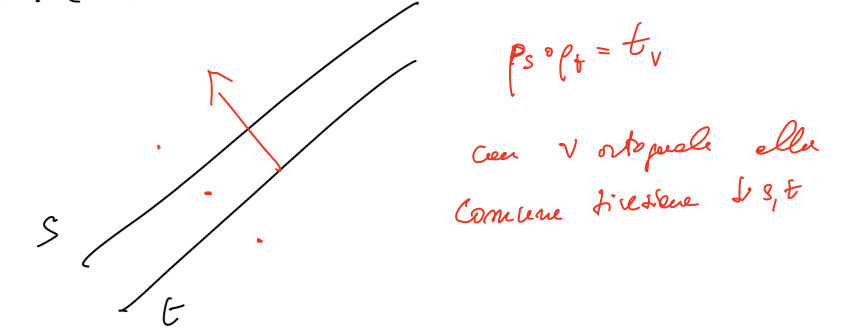
\includegraphics[scale=.4]{rette_parallele.png}\\
In coordinate rispetto ad un riferimetno cartesiano $Oe_1e_2$ Se $P\equiv\icol{x_1\\x_2}$ 
\[
	(R_{C,\theta}\circ R_{D,\varphi})(P) \ \ \ \text{ ha coordinate}
.\] 
\[
	R_\rho(R(x-d) + d-x) + x  
.\]
dove $c,d$ sono i vettori delle coordinate di $C,D $ rispettivamente\\
\begin{aligned}
	&\underline{R_{\theta + \varphi}(x - d)} + R_\theta(d-c) + c\\[-5px]
	&\hspace{-4px}\text{ parte lineare}
\end{aligend}\\[10px]
$T$ T è una translazione se e solo se $\theta + \varphi = 2k\pi, k\in\mathbb{Z}$ e in tal caso
\[
T(x) = x + R_\theta(d-c) = (d-c)
.\] 
che è l'identità se e solo se $d = c$ cioè $D=C$
\begin{defi}[Glissoriflessione]
	Una glissoriflessione è un'isometria di un piano euclideo ottenuta come composizione $t_v\circ\rho_r$ di una riflessione di asse $r$ con una traslazione $t_v\neq Id$ con $v\neq 0, v\parallel r$
\end{defi}
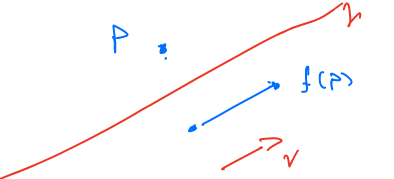
\includegraphics[scale=.4]{glissoriflessione.png}\\
\begin{teo}[Charles, 1831]
	Un'isometria di un piano euclideo che fissa un punto è una rotazione o una riflessione a seconda che sia diretta o inversa. Un'isometria senza punti fissi è una traslazione o una glissoriflessione a seconda che sia diretta o inversa
\end{teo}
\begin{dimo}
	Sia $f\in Isom(E)$\\ Se $f$ ha un punto fisso abbiamo già visto che $f$ è una rotazione se è diretta o una riflessione se $f$ è inversa\\
	se $f$ diretta priva di punti fissi. Allora anche $f^2$ non ha punti fissi, perché se $f^2(p) = p$ \\
	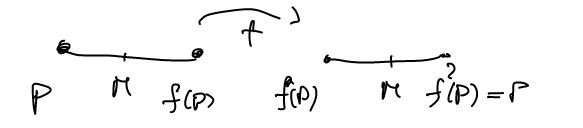
\includegraphics[scale=.4]{f_punti_fissi.png}\\
	Dunque $f(M) = M$ escluso.\\
	DIco che $p,f(p),f^2(p)$ che sono distinti per quanto abbiamo visto, sono allineati, Altrimneti  \\
	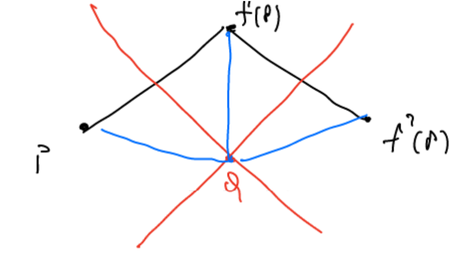
\includegraphics[scale=.6]{batman.png}
	\[
		d(P, f(p)) = d(f(p), f^2(p)) (\text{ poichè } f \text{ è un'isometria})
	.\] 
	\[
		d(Q,P) = d(Q,f(P)) = d(Q,f^2(P))
	.\] 
	Poiché $f$ preserva l'orientazione, il triangolo $QPf(P)$ viene trasformato in  $Q,f(P),f^2(P)$ da cui $f(Q) = Q$\\
	Dunque tutti i punti  $f^i(P), \ \ i\geq 0$ sono allineati, quindi se  $r$ è la retta che li contiene, $f$ agisce su $r$ come una traslazione.\\
	Poiché $f$ è diretta, $f$ agisce su tutto il piano come una traslazione.\\[10px]
	Sia ora $f$ inversa senza punti fissi,\\ Allora $f^2$ è diretta e come prima $f^2= t_v$ per qualche $v$\\
	Sia $P\in E$ un punto $r_0 = \overrightarrow{Pf^2(P)}, \ \ r_1 = \overrightarrow{f(P)f^2(P)}$ \\
	sono rette parallele che sono scambiate tra loro da $f$ \\
	\ \ \ \ 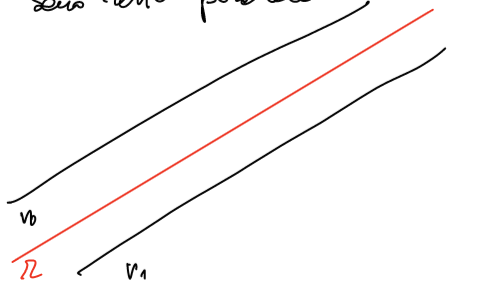
\includegraphics[trim={0 0 0 25px},clip,scale=.4]{rette_scambiate.png}\\
	Sia $r$ la retta equidistante da $r_0$ e $r_1$.\\ Allora $f(r)\subseteq r  $ Ma $f^2 = t_v$ 
	$f|_r = t_{v/2}$\\
	Se ora consideriamo $t_{-v/2}\circ f$ \\questa è un'isometria inversa che fissa puntualmente $r$,\\ quindi è una riflessione che indichiamo con $\rho$. Dunque
	\[
		f = t_{v/2}\circ t_{-v/2}\circ f = t_{ v/2}\circ \rho
	.\] 
\end{dimo}
\subsection{Diagonalizzazione di operatori simmetrici}
\textbf{Ricorda}\\
$f\in End(V) $ diagonalizzabile se esiste una base di $V$ di autovettori di  $f\\ \Leftrightarrow A = [f]^B_B$ B base $\exists N\in GL(n,\mathbb{K}): N^{-1}AN$ è diagonale 
\begin{lemm}
	Il polinomio caratteristico di $A\in M_n(\mathbb{R})$ simmetrica ha solo radici reali
\end{lemm}
\begin{dimo}
	$A\in M_n(\mathbb{R}) \subseteq(\mathbb{C}) \ \ L_A : \mathbb{C}^n \rightarrow \C ^n.\\$
	Sia $\lambda\in \C$ un autovalore e $x\neq 0$ un corrispondente autovettore 
	\[
	Ax = \lambda x
	.\] 
	\[
		\overline{Ax} = \overline{\lambda x}
	.\] 
	\[
		A\overline{x} = \overline{\lambda}\overline{x}
	.\] 
	$\overline{x}^tAx = \overline{x}^t(Ax) = \overline{x}^t(\lambda x) = \lambda \overline{x}^t x\\
	\overline{x}^t A x = \overline{x}^t A^t x = (A\overline{x})^tx = (\overline{\lambda}\overline{x})^tx = \overline{\lambda}\overline{x}^tx$\\
	$\overline{x}^tx = \sum^n_{i=1}\overline{x}_ix_i$ $\leftarrow$ è un numero reale positivo poiché $x\neq 0$
	\[
		\lambda \overline{x}^tx = \overline{\lambda}\oveline{x}^tx \ \ \ \Rightarrow \ \ \ \lambda = \oveline{\lambda}
	.\] 
\end{dimo}
\begin{teo}[Teorema Spettrale]
	Sia $V$ uno spazio euclideo di dimensione finita e $T\in End(V)$ un operatore simmetrico, esiste una bas ortonormale di autovettori per $T$
\end{teo}
\begin{coro}
	Per ogni matrice reale simmetrica $A\in M_n(\R)$ esiste una matrice ortogonale $N\in O(n)$ tale che 
	 \[
		 N^{-1}AM = N^tAN \ \ \ \ \ \text{ è ortogonale}
	.\] 
\end{coro}
\begin{dimo}[Teorema]
	 Per induzione su $n = dim(V)$. Base $n = 1$ ovvia\\
	 Supponiamo $n = dim(v) \geq 2$. Poichè $T$ è simmetrico il polinomio caratteristico ha radici reali (per il lemma precedente) quindi $T$ ammette un autovalore $\lambda$ d sia $e_1$ il suo corrispondente autovettore di lunghezza $1$
	 \[
	 V = \R e_1\oplus(\R e_1)^\perp
	 .\] 
	 Chiamo $U \equiv (\R e_1)^\perp$ \\Dico che $T|_U :U \rightarrow$, per cui $T|_U\in End(U)$\\
	 Infatti, dimostro che $u\in U \rightarrow T(u)\in U$\\
\textbf{ipotesi: } $ \langle u, e_1 \rangle = 0$\\
\textbf{Tesi:} $ \langle Tu, e_1 \rangle  = \langle u, T^te_1 \rangle = \langle u, Te_1 \rangle = \langle u, \lambda e_1 \rangle  = \lambda \langle u, e_1 \rangle  = 0$\\
dove abbiamo usato la simmetria di T\\
Chiaramente $T|_U$ è simmetrico, quindi per induzione $U$ ha una base ortonormale di autovettori $\{e_2,\ldots,d_n\}$.\\
Ne segue che $\{e_1,\ldots,e_n\}$ è una base ortonormale di $V$ formata da autovettori per $T$
\end{dimo}
\subsection{Prodotto Hermitiano}
	$V$ spazio vettoriale complesso
	\begin{defi}[Funzione sesquilineare]
		Una funzione sesquilineare su $V$ è un'applicazione $h: V\times V \rightarrow \mathbb{C}$\\
		che è lineare nella prima variabile e antilineare nella seconda, cioè\\[10px]
		\begin{aligned}
			\hspace{80px}&h(v+v',w) = h(v,w) + g(v',w)\\
		&h(\alpha v,w) = \alpha h(v,w)\\
		&h(v,w + w') = h(v,w) + h(v,w')\\
			&h(v,\alpha w) = \overline{\alpha}h(v,w)\\
		\end{aligned}\\[10px]
		per ogni scelta di $v,w,v',w'\in V$ e $\alpha \in\mathbb{C}$
	\end{defi}
	\begin{defi}[Forma hermitiana]
		Una forma sesquilineare si dice hermitiana se
		\[
			h(v,w) = \overline{h(w,v)}
		.\] 
	\end{defi}
	\textbf{Osservazione}\\
	Se $h$ è hermitiana, $h(v,v)\in\R$, infatti deve risultare $h(v,v) = \overline{h(v,v)}$
	\begin{defi}[Forma antihermitiana]
		Una forma sesquilineare si dice antihermitiana se 
		\[
			g(v,w) = - \overline{h(v,w)}
		.\] 
	\end{defi}
	\textbf{Osservazione}\\
	In questo caso $h(v,v)\in\sqrt{1}\R$\\
	\begin{defi}
		Una forma hermitiana si dice semidefinita positiva se 
		\[
		h(v,v) \geq 0 \ \ \forall v\in V
		.\] 
	\end{defi}
	\begin{defi}
		Una forma hermitiana si dice definita positiva se 
		\[
		h(v,v)>0 \ \ \forall v \neq 0
		.\] 
		ovvero
		\[
			(h(v,v)\geq 0 \text{ e }h(v,v) = 0 \Rightarrow v=0)
		.\] 
	\end{defi}
	\textbf{Esempio}\\
	$V = \C^n$
	\[
		h( \icol{z_1\\ \vdots \\ z_n},\icol{w_1\\\vdots\\w_n}) = \sum^n_{i=1}z_i\overline{w_i}
	.\] 
	questo viene chiamato prodotto hermitiano standard su $\C^n$
 \[
		h( \icol{z_1\\ \vdots \\ z_n},\icol{z_1\\\vdots\\z_n}) = \sum^n_{i=1}z_i\overline{z_i} = \sum^n_{i=1}|z_i|^2
	\]
	\newpage
	Dato $V$, consideriamo una base $B = \{v_1,\ldots,v_n\}$ di $V$ Se $h$ è una forma heritiana, diciamo che $(h_{ij}) = h(v_i,v_j)$ è la matrice che rappresenta $h$ nella base $B$ e la denoto come $(h)_B$\\
	se  $v = \sum^n_{i=1}x_iv_i, \ \ \ w = \sum^n_{i=1}y_iv_i$\\
\begin{aligned}
	\hspace{30px}h(v,w) &= h(\sum^n_{i=1}x_iv_i,\sum^n_{i=1}y_iv_i) = \\
&= \sum^n_{i=1}x_ih_i(v_i,\sum^n_{i=1}y_iv_i) = \\
& = \sum^n_{i=1}x_i\overline{y_i}h(v_i,v_i) = \\
& = x^t H\overline{y}
\end{aligned}\\
Poiché $h$ è hermitiana, $h(v,w) = \overline{h(w,v)}$\\
\begin{aligned}
	X^tHY &= \overline{Y^tHX}\\
	 &     = \overline{Y}^t \overline{H} \overline{X}\\
	 & = (\overline{Y}^t \overline{H} \overline{X})^t\\
	 & = \overline{X}^t \overline{H}^t \overline{Y} \ \ \ \ \Rightarrow \ \ \  H = \overline{H}^t
\end{aligned}
\begin{defi}
	Una matrice $M\in M_n(\C)$ si dice hermitiana se
	\[
		H = \overline{H}^t
	.\] 
\end{defi}
\textbf{Esercizio}\\
le matrici hermitiane $2\times 2$ sono un $\R$-sottospazio di $M_2(\C)$ di dimensione 4
\[
	\matrice{a_1 + ib_1 & a_2 + ib_2\\ a_3 + ib_3 & a_4 + ib_4} = \matrice{a_1 - ib_1 & a_3 - ib_3\\a_2 - ib_2 & a_4 - ib_4}
.\] 

$\Rightarrow \hspace{20px}$\begin{aligned}
	& a_1 + ib_1 = a_1 - ib_1 \Rightarrow  b_1 = 0\\
	&a_2 + ib_2 = a_3 - ib_3 \Rightarrow  a_2 = a_3 \ \ b_2 = -b_3\\
	&a_3 + ib_3 = a_2 - ib_2\Rightarrow  a_2 = a_3 \ \ b_2 = -b_3\\
	&a_4 + ib_4 = a_4-ib_4 \Rightarrow b_4 = 0\\[10px]
\end{aligned}\\
\begin{aligend}
	&\matrice{a_1&a_2+ib_2\\a_2-ib_2&a_4}\\[10px]
	&M_2 = \R\icol{1&0\\0&0}\oplus\R\icol{0&0\\0&1}\oplus\R\icol{0&1\\1&0}\oplus\R\icol{0&i\\-i&0}
\end{aligend}\\
\newpage
Si definiscano allo stesso modo del caso reale simmetrico $S^t$\\
coefficiente di Fourier
\[
| \langle v, w \rangle |\leq ||v||||w||
.\] 
disuguaglianza triangolare $||v+w||\leq||v|| + ||w||$\\
Operatore unitario: $T\in End_\C(V)$ t.c.
\[
\langle T(u), T(v) \rangle  = \langle u, v \rangle \ \ \ \forall u,v\in V
.\] 
Verifichiamo le caratteristiche degli operatori unitari dati nel caso reale\\
\textbf{Gram Schmidt}\\
$T\in End(V)$ operatore unitario\\
$1.$ Gli autovalori hanno modulo 1\\
$2.$ Autospazi relativi ad autovalori distinti sono ortogonali\\
$1.$ Sia $v$ un autovettore di autovalore $\lambda$ 
\[
	\langle v, v \rangle = \langle Tv, Tv \rangle  = \langle tv, tv \rangle  = \lambda\overline{\lambda} \langle v, v \rangle = |\lambda|^2 \langle v, v \rangle 
.\] 
\[
v \neq 0 \Rightarrow  \ \ \ |\lambda|^2 = 1 \ \ \  \Rightarrow  \ \ \ |\lambda| = 1
.\] 
$2.$ Sia $v\in V_\lambda$, $w\in V_\mu$ \ \ $\lambda\neq\mu$
\[
	\langle v, w \rangle  = \langle Tv, Tw \rangle = \langle \lambda v, \mu w \rangle = \lambda\overline{\mu} \langle v, w \rangle 
.\] 
Se $ \langle v, w \rangle \neq 0 $ \neq 0 \Rightarrow \lambda \overline{\mu} = 1$. Per il punto 1\\
\[
	\lambda\overline{\lambda} \ \ \Rightarrow \ \ \overline{\lambda} = \overline{\mu} \ \ \Rightarrow \ \ \lambda = \mu \ \ \text{ assurdo}
.\] 
\begin{defi}
	Diciamo che $U\in M_n(\C)$ è unitaria se 
	\[
		U\overline{U}^t = Id
	.\] 
\end{defi}
\begin{prop}
	$T\in End(V)$ è unitario se e solo se la sua matrice in una base ortonormale è unitaria
\end{prop}
\begin{dimo}
	Sia $B = \{v_1,\ldots,v_n\}$ una base ortonormale di $V$ 
	\[
		\delta_{ij} = \langle v_i, v_j \rangle  = \langle Tv_i, Tv_j \rangle  = \langle Ae_i, Ae_j \rangle = e_i^tA^t\overline{A}e_j = A_i^t\overline{A}_j
	\] 
	dove abbiamo posto $A = (T)_B$ e $\{e_i\}$ è una base di $\C^n$\\
	w dove $A_{i}, A_{j}$ sono la $i$-esima e la $j$-esima colonna di $A$\\
	($A_i^t\overline{A}_j$ è il prodotto hermitiano standard)
\end{dimo}\\
Come nel caso reale si dimostra
\begin{teo}
	Sia $T\in End(V)$ un operatore unitario Esiste una base standard di autovettori per $T$
\end{teo} 
In particolare, per ogni matrice unitaria $A\in U(n)$ esiste $M\in U(n)$ tale che $M^{-1}AM$ è diagonale
\begin{nota}
	a volte si pone 
	\[
	 A^* = \overline{A}^t
	.\] 
	$A$ unitario $AA^* = Id$ \\
	$A$ hermitiano $A = A^*$ \\
	$A$ antihermitiano $A=-A^*$
\end{nota}
\begin{defi}[Operatore Aggiunto]
	Dato $T\in End(V)$, esiste unico $S\in End(V)$ tale che 
	\[
	\langle Tu, w \rangle = \langle u, Sw \rangle \ \ \forall u,w\in V
	.\] 
	Tale operatore è detto aggiunto hermitiano di $T$ e denotato con $T^*$
\end{defi}
\begin{defi}[operatore normale]
	Sia $V$ uno spazio vettoriale complesso dotato di prodotto hermitiano (forma hermitiana definita positiva), un operatore $L\in End(V)$ è normale se 
	\[
	L\circ L^* = L^*\circ L
	.\] 
\end{defi}
\textbf{Osservazione}\\
$L$ unitario, hermitiano, antihermitiano $ \Rightarrow$ $L$ diagonale
\begin{teo}
	Sono equivalenti le seguenti affermazioni:\\
	$1)$ $L$ è normale\\
	$2)$ esiste una base ortonormale di $V$ formata da autovettori di $L$
\end{teo}
\newpage
	\subsection{Diangonalizzazione unitaria di operatori normali}
	($\C^n$, prodotto hermitiano standard) $M^\star = \overline{M}^t$\\
	 $M$ è normale se $MM^\star = M^\star M$\\
	 siano normali le matrici\\ \begin{aligned}
		 \hspace{120px}&\text{unitarie} \ \ \ \ &MM^\star = Id\\
						       &\text{hermitiane} \ \ \ \ &M=M^\star\\
						       &\text{antihermitiane} \ \ \ &M = -M^\star
	 \end{aligned}\\
	 \begin{teo}[Spettrale]
	 	$M$ è normale se e solo se $\exists U\in U(n) : \ U^tMU$ è ortogonale
	 \end{teo}
	 \textbf{Nota}\\
	 $U(n)$ spazio delle matrici unitarie\\$
	 \subsection{Classificazioni delle isometrie}
	 \begin{nome}
	$\cdot$ rotazioni\\
	$\cdot$ riflessioni\\
	$\cdot$ traslazioni\\
	$\cdot$ glissoriflessione $ = t_v\circ s_\alpha$ con $v\parallel \alpha^t$ (disegno de li mortacci sua)\\
$\cdot$ glissorotazioni $= t\circ R$ dove $v \parallel a$, $a$ asse di $R$ (altro disegno)\\
$\cdot$ riflessioni rotatorie $s_a\circ R$  $R$ rotazione di asse $\underline{a}$,  $s_\underline{a}$ è una riflessione rispetto ad una retta parallela ad $\underline{a}$
\end{nome}
\begin{teo}[Eulero 1776]
	Ogni isometria di $\mathbb{E}^3$ è di uno dei sei tipi sopra descritti
\end{teo}
\subsection{Teoremi vari su spazi Hermitiani e company}
	\begin{lemm}
		Sia $V$ uno spazio vettoriale su un campo $\R$\\
		Siano  $P,Q\in End(V)$ tali che $PQ=QP$. Allora, se  $V_\lambda$ è l'autospazio di autovalore $\lambda$ su $P$, risulta
		\[
		Q(V_\lambda)\subseteq V_\lambda
		.\] 
	\end{lemm}
	\begin{dimo}
		Sia $v\in V_ \lambda $ (cioè $P(v) = \lambda v)$. Dobbiamo vedere che $Qv\in V_ \lambda$.
		\[
		P(Q(v)) = (P\circ Q)(v) = (Q\circ P)(v) = Q( \lambda v) = \lambda Q(v)
		.\]
	\end{dimo}
	$(V,h)$ spazio Hermitiano (Spazio vettoriale complesso $h$ forma hermitiana definita positiva in $V$ )\\
	$\dim(V) < +\infty$
	 \begin{teo}
		Sia $(V,h)$ uno spazio hermitiano, $L\in End(V)$ operatore, sono equivalenti
		\begin{itemize}
			\item $L$ è normale (rispetto ad $h$)
			\item esiste una base ortonormale $B$ di  $V$ composta da autovettori per $L$
		\end{itemize}
	\end{teo}
	\begin{lemm}
		$(V,h)$ spazio hermitiano, $L\in End(V)$ normale\\
		sono equivalenti
		\begin{itemize}
			\item $Lv = \lambda v$
			\item  $L^\star v = \overline{ \lambda} v$
		\end{itemize}
		In particolare $ \lambda$ è l'autovalore per $L$ se e solo se $\overline{ \lambda}$ è autovalore per $ L^\star$ 
		\[
			V_ \lambda (L) = V_{\overline{ \lambda}}(L^\star)
		.\] 
	\end{lemm}
	\begin{dimo}
		Se $v = 0$ non c'è niente da dimostrare.\\
		Se $v \neq 0$ basta far vedere che se $v\in V_ \lambda (L)$ allora $v\in V_{\overline{ \lambda}}(L^\star)$. L'inclusione contraria segue da $L^{\star t} = L$
		 \[
		w\in V_ \lambda (L), \ \ v\in V_ \lambda (L)
		.\] 
		\begin{aligned}
			\hspace{80px}h(L^\star(v),w) &= h(v,L(w)) = h(v, \lambda w)\\
					&=\overline{ \lambda}h(v,w) = h(\overline{ \lambda}v,w)
		\end{aligned}\\
		\[
			h(L^\star(v) - \overline{ \lambda}v,w) = 0 \ \ \circledast
		\] 
		Per il lemma, siccome per ipotesi $L$ è normale, 
		 \[
		L^\star (v)\in V_\lambda (L), \ \ \overline{
		\lambda}v\in V_ \lambda (L)
		\] 
		\[
			\Rightarrow \ \ \ L^\star (v) - \overline{ \lambda} v\in V_ \lambda (L)
		\] 
		Quindi nella $\circledast$ posso prendere $w = L^\star (v) - \overline{ \lambda} v$, ottenendo 
		\[
			h(L^\star (v) - \overline{ \lambda} v, L^\star (v) - \overline{\lambda} v) = 0
		.\] 
		Poiché $h$ è definito positivo, segue\\
		\begin{aligned}
			&L^\star(v) - \overline{ \lambda}v = 0\\
			\text{cioè} \hspace{50px}  & L^\star (v) = \overline{ \lambda} v
		\end{aligned}\\
	\end{dimo}
	\textbf{Osservazione}\\
	Dal lemma segue $V_ \lambda(L) \perp V_\mu (L)$ se $ \lambda \neq \mu$
	\[
	v\in V_ \lambda, \ \ \ w\in V_\mu
	\] 
	\[
		\lambda h(v,w) = h( \lambda v,w) = h(Lv,w) = h(v,L^\star w) = h(v, \overline{\mu}w) = \mu h(v,w) \Rightarrow  h(v,w) = 0
	\]
	Dato che $ \lambda \neq \mu$
	\begin{dimo}[Teorema Spettrale]
		$1) \Rightarrow  2)$ Procediamo per induzione su $\dim V$,con base ovvia $\dim V = 1$ \\
		Supponiamo il teorema vero per gli spazi hermitiani di dimensione $\leq n-1$ e sia  $\dim_\C V = n$\\
		Sia  $v_1\in V$ un autovettore per $L$, che possiamo assumere di norma  $1$. Sia $V_1 = \C v_1, W = v_1^perp$.\\
		Allora $V = V_1 \oplus W$.\\
		Poiché $V_1$ è $L$-invariante (per costruzione) e $L^\star$-invariante per il lemma precedente, lo stesso accade per  $W$.\\
		Inoltre $L|_W\in End(V)$ è normale.\\
		Per induzione, esiste una base $h|_W$-ortonormale formata da autovettori per $L|_W$, sia $\{v_2,\ldots,v_n\}.$ Allora $\{v_1,\ldots,v_n\}$ è una base $h$-ortonormale di $V$ formata da autovettori per $L$.\\
		$2) \Rightarrow 1)$. Sia $B = \{v_1,\ldots,v_n\}$ una base $h$-ortonormale di autovettori per $L$. Allora\\
		\begin{aligned}
			\hspace{80px}&[L]^B_B = \bigwedge = \matrice{ \lambda_1  &\ldots& 0\\
				 0  & \ddots & 0\\
			 0  &\ldots & \lambda_n}\\
			    &[L^\star]^B_B = \overline{[L]_B^B}^t = \overline{\bigwedge}\\
			    &[L\circ L^\star]^B_B = [L]^B_B[L^\star]^B_B = \bigwedge\overline{\bigwedge}=\overline{\bigwedge}\bigwedge = [L^\star]_B^B[L]^B_B = [L^\star \circ L]_B^B
		 \end{aligned} \\
		 Poiché la mappa $A \rightarrow [A]^B_B$ è un isomorfismo tra
		 $End(V)$ e $M_{nn}(\C)$, segue 
		 \[
		 L\circ L^\star = L^\star \circ L
		 .\] 
		 cioè $L$ è normale
	\end{dimo}
	\textbf{Osservazioni}\\
	1. È essenziale che $h$ sia definita positiva.\\
	\[
	 h(x,y) = x^tH\overline{y} \ \ \ M = \matrice{1&0\\0&-1}
	.\] 
	non è definita positiva $h(\icol{0\\1},\icol{0\\1}) = -1$
	\[
		L_A:\C^2 \rightarrow\C^2 \ \ A = \matrice{0&i\\i & -2}
	.\] 
	Dico che $L_A$ è autoaggiunto, quindi normale\\
	\begin{aligned}
		\hspace{80px}&h(L_AX,Y) = h(X,L_AY)\\
		&(L_AX)^tH\overline{Y} = X^tH\overline{L_AY}\\
		&X^tA^tH\overline{Y} = X^tH\overline{A}\overline{Y} \ \ \forall X,Y\\
		&A^tH = H\overline{A}\\
		&\matrice{0&u\\i&-2}\matrice{1&0\\0&-1} = \matrice{1&0\\0&-1}\matrice{0&-i\\-i&-2}\\
		&\hspace{47px}\matrice{0&-i\\i&2} = \matrice{0&-i\\i&2}
	\end{aligned}\\
	Calcolo il polinomio caratteristico di $A$ 
	\[
		\det\matrice{t& -i\\-i & t + 2} = t(t+2) + 1 = (t+1)^2
	.\] 
		Ma $A\neq \matrice{-1&0\\0&-1}$, in particolare non è diagonalizzabile\\
		2. Vediamo in dettaglio il fatto che $L|_W$ è normale\\
		Ritornando alla dimostrazione del teorema spettrlae, osserviamo che se $W$ è $L$-invariante è anche $L^\star$-invariante.\\
		Infatti, se $V = \bigoplus_\lambda V_ \lambda(L)$ (per esercizio da dimostrare)\\
		\begin{aligend}
			$W &= \bigoplus_ \lambda (V_ \lambda(L)\cap W)$\\
			   &=\bigoplus_ \lambda (V_{\overline{ \lambda}}(L^\star)\cap W)
			
		\end{aligend}\\
		$=> W$ è $L^\star$-invariante\\
		Adesso osservo che $(L|_W)^\star = (L^\star)|_W$\\
		\begin{aligend}
			&(L\left|_{W)}\circ(L\right|_W)^\star = (L|_W)\circ(L^star|_W) = \\
			&(L\circ L^\star)|_W = (L^\star\circ L)|_W = (L^\star|_W) \circ L|_W = (L|_W)^\star\circ L|_W
		\end{aligend}\\
		\subsection{Richiami su spazi vettoriali duali}
		$V$ spazio vettoriale su $\K$ di dimensione finita
		 \[
		V^V = V^\star = Hom(V,\K)
		.\] 
		sia $A\leq V$
		 \[
			 Ann(A) = A^\# = \{f\in V^\star | f(a) = 0 \ \ \forall a \in A\}
		.\] 
		\textbf{Osservazioni}\\
		1) $A^\# $ è un sottospazio\\
		2) $A^{\#\#} = <A>$ \\
		\begin{aligned}
			\hspace{100px}&i:V \rightarrow V^{\star\star}\\
			&v\in V, \ \ f\in V^\star\\
			& i(v)(f) = f(v)
		\end{aligned}\\
	$V,W$ spazi vettoriali di dimensione finita $f\in Hom_\K(V,W)$, $f^\star\in Hom_\K(W^\star,V^\star)$, la trasposta di f è definita con $\phi\in W^\star$\\
	\hspace{40px}$f^\star(\phi) = \phi\circ f \\
	$\text{ }\hspace{100px}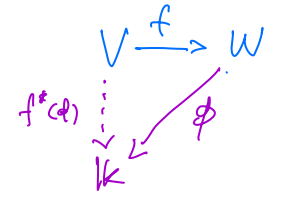
\includegraphics[scale=0.4]{funzione.png}\\
	\newpage
	\begin{defi}
	Definisco la  dualità standard su $V$ come 
	\[
	\langle \ , \  \rangle : V^\star\times V \rightarrow \K
	.\] 
	$\langle v, f \rangle = \langle f, v \rangle = f(v)$\\
	con questa proprietà
	\[
	\langle f(v), w^\star \rangle  = \langle v, f^\star(w^\star) \rangle 
	.\] 
\end{defi}
\hline \ \\
Ricordo che se $B = \{v_1,\ldots,v_n\}$ è una base di $V$ allora i funzionali $v_i^\star$ definiti da
 \[
	 \langle v_i^\star, v_j \rangle =\delta_{ij}
.\] 
per $1\leq i\leq n$ formano una base $B^\star$ di $V^\star$ detta base duale di $B$\\
Sia  $f:V \rightarrow W$ un'applicazione lineare, siano $B =\{v_1,\ldots,v_n\}, L = \{w_1,\ldots,w_m\}$ basi di $V,W$ consideriamo  $f^\star :W^\star \rightarrow V^\star$ Allora:\\
\begin{aligned}
	\hspace{120px}[f&]_B^B = [f^\star]^{B^\star}_{L^\star}^t	\\
		       & \storto{=} \ \ \ \hspace{18px} \storto{=}\\
		       &\hspace{-10px}(a_{ij}) \ \ \ \  (a^\star_{ij})
		        
\end{aligned}\\
\textbf{Tesi} \ \ $a_{ih} = a^\star_{hi}$\\
$f^\star(w^\star_i) = \sum^n_{i=1}a_{ij}^\starv_i^\star$\\
$f^\star(w_i^\star)(v_h) = \sum^n_{i=1}a^\star_{ij}v^\star_i(v_h) = \sum^n_{i=1}a_{ij}^\star\delta_{ih} = a^\star_{hi}$\\
\text{ }\ \ \storto{=}\\
$w_i^\star(f(w_h)) = w^\star_i(\sum^n_{i=1}a_{ih}w_i) = \sum^n_{i=1}a_{ih}w^\star_i(w_i)=$\\
$=\sum^n_{i=1}a_{ih}\delta_{ij}= a_{ih} $
\begin{teo}[Qualche proprietà importante]
	$f:V \rightarrow W$ lineare $\ \ f^\star : W^\star \rightarrow V^\star$\\
	$1) (Im f)^\# = \ker f^\star \\$
	 $2) (\ker f)^\# = Im f^\star$\\
	 $3) (\lambda f + \mu g)^\star = \lambda f^\star + \mu g^\star \ \ \ \ \ \ ( \lambda,\mu \in \K, g\in Hom(V,W)) $\\
	 $4) (h\circ f)^\star = f^\star\circ h^\star \hspace{40px} \ \ \ h:W \Rightarrow U $ lineare
\end{teo}
\begin{dimo}[Il punto 2, 3 e 4 vengono lasciati per esercizio]
	\begin{aligend}
	&1) $\emptyset\in (Im f)^\# $\\
	& \Leftrightarrow \forall w\in Imf \ \ \emptyset(w) = 0 \\
	& \Leftrightarrow \forall v \in V \emptyset(f(v)) = 0\\
	& \Leftrightarrow \emptyset \circ f = 0\\
	& \Leftrightarrow \emptyset \in kerf^\star
	\end{aligend}\\
	Quindi abbiamo visto che $(Imf)^\# = \ker F^\star$
\end{dimo}
\begin{prop}
	Sia $V$ uno spazio vettoriale di dimensione $n$ su $\K$ e $W$ un sottospazio. Allora
	\[
	\dim(W) + \dim W^\#  = n
	.\] 
\end{prop}
\begin{dimo}
	Da quanto visto, la mappa\\
	\begin{aligned}
		\hspace{80px}&Hom(V_1,V_2) \rightarrow Hom(V^star_2,V^star_1)\\
			     & \hspace{20px} \ f \ \ \ \ \ \ \ \  \rightarrow \ \ \  \ \ \ f^t
	\end{aligned}\\
	è un isomorfismo di spazi vettoriali. Inoltre $f$ è iniettiva (rispettivamente suriettiva) se e solo se $f^\star$ è suriettiva (rispettivamente iniettiva)\\
	Consideriamo la proiezione  $\pi:V \rightarrow V|_W :=U$ \\
	Poiché $\pi$ è suriettiva $\pi ^\star : U ^\star \rightarrow V^\star$ è iniettiva e 
	\[
	W^\#  = (\ker\pi)^\# = Im\pi^\star
	.\] 
	per cui 
	\[
	 \dim W^\# = \dim (Im \pi ^\star) = \dim U^\star = \dim V - \dim W
	.\] 
\end{dimo}

	\subsection{Forme bilineari 2}
	$V$ spazio vettoriale su $\R$ \\
	Ricordiamo che una forma bilineare è un'applicazione 
	\[
	b:V\times V \rightarrow \R
	.\] 
	Abbiamo già osservato che se $A = [b]_B$\\
	$X = [v]_B, \ \ Y=[w]_B$
	 \[
	b(v,w) = X^tAY
	.\] 
	Come cambia $[b]_B$ se cambio $B$ \\
	$B = \{v_1,\ldots,v_n\}$ \ \ \  X=[v]_B \ \ X'=[v]_B'\\
	$B' = \{v_1',\ldots,v_n'\}$ \ \ Y = [w]_B \ \ Y' = [w]_B'\\
	$A = [b]_B \ \ A' = [b]_{B'}$\\
	$$b(v,w) = X^tAY = X'^TA'Y'$$
	$X = MX', \ \ Y=MY'\ \ \ M = [Id_V]_B^B$\\
	 \begin{aligend}
		 \hspace{80px} &(MX')^tA(MY') = X'^t A'Y'\\
		 &X'M^t AMY' = X'^tA'Y'\\
		 & \ \ \ A' = M^tAM
	 \end{aligend}\\
\begin{defi}
	Diciamo che due matrici $A,B$ sono congruenti se esiste una matrice invertibile $M$ tale che  $B = M^tAM$
\end{defi}
\begin{prop}
	Due matrici rappresentano la stessa forma bilineare in basi diversi se e solo se sono congruenti
\end{prop}
\textbf{Osservazione}\\
1. La congruenza è una relazione di equivalenza\\
2. Il rango è invariante per la congruenza\\
3. Per matrici reali invertibili, il segno del determinante è invariante\\
4. Se $M$ è ortogonale\\
\[
	M^tAM = M^{-1}AM
.\] 
\hline \ \\
Se ho una forma bilineare $b:V\times V \rightarrow \mathbb{K}$ posso definire due applicazioni $V \rightarrow V^\star$ nel modo seguente.\\
Fissato $v\in V$, \ prendo \ \  \begin{aligned}
	&b_v(w) = b(v,w)\\
	&b_v'(w) = b(w,v)
\end{aligned}\\
È chiaro che $b_v, b'_v\in V^\star$ (usiamo il fatto che $b$ è bilineare)\\
Dunque ho due applicazioni $V \rightarrow V^\star$
\[
\delta_b(v) = b_v  \ \ \ \delta_b '(v) = b'_v
.\] 
\begin{defi}
	Il rango di una funzione bilineare è il rango di una qualsiasi matrice che la rappresenta
\end{defi}
\begin{defi}
	Una forma bilineare è non degenere se ha rango (massimo) $\dim V$
\end{defi}
\newpage
\begin{prop}
Sia $V$ uno spazio vettoriale di dimensione finita,
\[
	b:V\times V \rightarrow \K \text{ una forma bilineare}
.\] 
Sono equivalenti 
\begin{itemize}
	\item $b$ è non degenere ovvero $b(v,v)= 0 \Leftrightarrow v = 0$
	\item $\forall v\in V, v\neq 0\ \ \exists w\in V : \ \ b(v,w)\neq 0$
	\item $\forall w\in V, \ w\neq 0 \ \ \exists v\in V: b(v,w) \neq 0$
	\item $\delta_b :V \rightarrow V^\star$ è un isomorfismo
	\item $\delta_b' : V \rightarrow V^*$ è un isomorfismo
\end{itemize}
\end{prop}
\begin{dimo}
	Sia $B = \{v_1,\ldots,v_n\}$ una base di $V$ e sia $A = [b]_B$\\
	$1) \Rightarrow  2)$ per ipotesi $\det A \neq 0$ se  $X = [v]_B \ \ X\neq 0  \Rightarrow  X^tA\neq 0$ \\
	quindi esiste $Y\in \K^n: X^tAY\neq 0$.\\ Se  $w\in V$ è tale che $[w]_B=Y$ ho dimostrato che  $b(v,w) = X^tAY\neq 0$ \\
	$2) \Rightarrow 1)$ Riscrivendo l'ipotesi in coordinate abbiamo\\
	\begin{aligned}
	\hspace{80px}&\forall X\neq 0 \ \exists Y : \ \ X^tAY\neq 0	\\
	& \Rightarrow X^t A\neq 0 \ \ \forall X\neq 0 \Rightarrow  A \text{ è invertibile}
	\end{aligned}\\
	$1) \Leftrightarrow 3)$ è come sopra\\
	$2) \Rightarrow 4)$ Poiché $\dim V = \dim V^\star$ basta vedere che $\delta_b$ è iniettava, cioè  $\ker\delta_b=\{0\}$\\
	 \begin{aligend}
		&v\in \ker\delta_b \ \ \Rightarrow \ \ \delta_b(v) = b_v \ \text{ è il funzionale nullo, cioè}\\
		&b_v(w) = 0 \ \ \forall w\in V\\
		&b_v(w) = b(v,w) \Rightarrow  v = 0 
	\end{aligend}\\
	$4) \Rightarrow  2)$ Dato $v\neq 0$,  $\delta_b(v) = b_v\neq 0$ perché  $\delta_b$ è un isomorfismo, \\quindi esiste  $w\in V:$\\
	\[b(v,w) = b_v(w)\neq 0\]
	$3) \Leftrightarrow 5)$ è simile a $2) \Leftrightarrow 4)$
\end{dimo}
\subsection{Caso Simmetrico}
\[
b(v,w) = b(w,v)
.\] 
\textbf{Osservazione}\\
$b$ è simmetrica se e solo se lo è qualsiasi matrice che la rappresenta.
\textbf{Dato} $S\subset V$ definiamo
\[
	S^\perp = \{v\in V| b(v,s) = 0 \ \ \forall s\in S\}
.\] 
\textbf{Esercizio} $S^\perp$ è un sottogruppo e, $S^\perp = <s>^\perp$
\begin{defi}
	Due sottospazi $U,W$ si dicono ortogonali se\\
	\[
	Y\subseteq W^perp \ \( \Leftrightarrow W\subset U^\perp )\\\]
\end{defi}
\begin{defi}
	$v\in V$ si dice isotropo se $b(v,v) = 0$\\
\end{defi}
\begin{defi}
	$\ker b = \{ v\in V|b(v,w)=0 \ \ \forall w\in V\} = V^\perp$
\end{defi}
 \textbf{Osservazione}\\
 $b$ è non degenere se e solo se $\ker b = \{0\}$\\
 \begin{prop}
 	Sia $b$ non degenere, $W\subseteq V$ sottospazio,\\
	Allora, se $\delta_b:V \rightarrow V^\star$ è l'isomorfismo canonico indotto da $b$, $\delta_b(W^t) = W^\star.$ In particolare risulta sempre $\dim W + \dim W^\perp = \dim V$
 \end{prop}
 \textbf{Nota}\\
 Non è vero, anche nel caso non degenere, che $V = W\oplus W^\perp$
\begin{dimo}
	$w\in W^\perp\ \ \ \delta_b(w) = b_w$ Voglio vedere che\\
	$b_w\in W^\# \ \ \ b_w(w')=b(w,w')=0 \ \ \forall w'\in W$ \\
	Quindi $\delta_b(W^\perp)\subseteq W^\#$\\
	Prendo ora  $f\in W^\# $; poiché  $b$ è non degenere, $\delta_b$ è un isomorfismo, quindi esiste $v\in V$
	 \[
	f = \delta_b(v) = b_v \ \ b(v,w) = b_v(w) = 0 \ \ \forall w \Rightarrow v\in W^\perp
	.\] 
	quindi $f = \delta(b_v)$ con $v\in W^\perp$
\end{dimo}
\begin{prop}
	Sia $V$ spazio vettoriale, $W\subset V$ sottospazio, $b\in Bi(V).$ Sono equivalenti:
	\begin{itemize}
		\item $V = W\oplus W^\perp$ 
		\item $b|_W$ è non degenere
	\end{itemize}
\end{prop}
\newpage
\begin{lemm}
	$\ker b|_W = W\cap W^\perp$
\end{lemm}
\begin{dimo}[lemma]
	$w\in \ker b|_W \Leftrightarrow b(w,w') = 0 \ \ \forall w'\in W \Leftrightarrow w \in W\cap W'$
\end{dimo}
\begin{dimo}[proposizione]
	$1) \Rightarrow 2)$segue dal lemma perché dall'ipotesi $W\cap W^\perp = \{0\}$ \\
	$2) \Rightarrow  1)$ Sia $\{w_1,\ldots,w_s\}$ una base di $W$ \\
	Per ipotesi $A = (b(w_i,w_j))$ è invertibile, in particolare dato $v\in V$, il sistema lineare
	\[
		* \ \ A\matrice{x_1\\\vdots\\x_s} = \matrice{b(v,w_1)\\\vdots\\b(v,w_s)}
	\]
	ha soluzione unica. Poniamo 
	\[
	w = v - \sum^s_{h=1}x_jw_j
	.\] 
	Notiamo che * significa
	\[
	\sum^s_{h=1}b(v_h,w_j)x_h=b(v,w_j) \ \ 1\leq j \leq s
	.\] 
	Calcoliamo \\
	\begin{aligned}
		&b(w,w_i) = b(v - \sum^s_{h=1}x_hw_h, w_j) =  b(v,w_j) - \sum^s_{h=1}x_hb(w_h,w_j) = b(v,w_j) = \\
		&=b(v,w_i) - b(v,w_i) = 0
	\end{aligned}\\
	Poiché i $\{w_i\}$ sono una base di $W$, risulta $b(w,u) = 0\ \ \ \forall u\in W$, cioè  $w\in W^\perp$ Allora
	\[
	v = w + \sum^s_{h=1}x_hw_h
	.\] 
	Pertanto $V = W + W^\perp$, per ipotesi  $W\cap W^\perp = \ker b|_W = \{0\}$, quindi $V = W\oplus W^\perp$
\end{dimo}
\subsection{Sylvester e forme quadratiche}
\begin{defi}
	 	la forma quadratica associata a $V$ è l'applicazione $q:V \rightarrow \K$ definita da $q(v) = g(v,v)$ e questa è una funzione omogenea di grado $2$
	 \end{defi}
	 \textbf{Esempio}\\
	 $V\cong \K^n, g = $ prodotto scalare standard\\
	 $g\matrice{x_1\\\vdots\\x_n} = \sum^n_{i=1}x_i^2$\\
	 \textbf{Osservazione}\\
	 Valgono:\\
	 1) $q(kv) = k^2q(v)$ \\
	 2) $2g(v,w) = q(v+w) - q(v) - q(w)$\\
	 dove $g(v,w)$ è la forma polare di $q$
	  \begin{dimo}
		  1.\hl{$q(kv)$}$= g(kv,kv) = k^2g(v,v) =$ \hl{$k^2q(v)$}\\
		  2.\hl{$q(v+w)- q(v)-q(w)$} $=g(v+w,v+w) - g(v,v)-g(w,w)= \\
		  =\cancel{g(v,v)}+2g(w,v)+\cancel{g(w,w)}-\cancel{g(v,v)}-\cancel{g(w,w)}= $ \hl{$2g(w,v)$}
	 \end{dimo}
	 \textbf{Osservazione}\\
	 $V=\R^4$ e sia $q\icol{x_1\\x_2\\x_3\\x_4}= x_1^2+2x_2^2-x_4^2+x_1x_4+6x_2x_3-2x_1x_2$\\
	 Voglio trovare la matrice della forma polare di $q$ rispetto  alla base canonica\\
	 $\matrice{1&-1&0&1/2\\-1&2&3&0\\0&3&0&0\\1/2&0&0&-1}$\\
	 Sulla diagonale ci sono i coefficienti delle componenti al quadrato  $(x_i)^2$ gli altri li ottieni dividendo per 2 ogni altro coefficiente 
	\\
	\begin{teo}[(Caratteristica di $\K)\neq 2$]
		Dato $V$ spazio vettoriale di dimensione $n\geq 1$ e  $g$ forma bilineare simmetrica su $V $, allora esiste una base $g$-ortogonale.
	\end{teo}
	\begin{dimo}
		Per induzione su $\dim V = n$. Se  $n=1$ non c'è nulla da dimostrare.\\
		se $g$ è la forma bilineare nulla ($g(v,w)=0 \ \ \forall v,w\in V)$ ogni base è  $g-$ortogonale.\\
		Altrimenti esistono,  $v,w\in V$ con $g(v,w)\neq 0$.\\
		Assumo che almeno uno tra  $v,w,v+w$ è non isotropo. Infatti se $v,w$ sono isotropi
		\[
		g(v+w,v+w)=g(v,v) + g(v,w) + g(w,w) = 2g(v,w)\neq 0)
		.\] 
		quindi $\exists v_1\in V$ t.c $g(v_1,v_1)\neq 0$. Allora $g|_{\K v_1}$ è non degenere quindi $V = \K v_1\oplus W$ con $W = (\K v_1)^\perp$ \\
		$\dim(W) = n-1$, per induzione $\exists$ una base  $\{v_2,\ldots,v_n\}$ di $W$ con $g(v_1,v_j) = 0$ se $2\leq j\leq n, \{v_1,\ldots,v_n\}$ è una base $g$-ortogonale di $V$
	\end{dimo}
	\begin{teo}
		Supponiamo $\K$ algebricamente chiuso. Sia $V$ spazio vettoriale dimensione $n\geq 1$ e $g$ forma bilineare simmetrica su $V$, esiste una base di $V$ rispetto alla quale la matrice di $g$ è $D=\matrice{I_r&0\\0&O_{n-r}}$ r = rg(D)\\
In modo equivalente, ogni matrice simmetrica a coefficienti in  $\K$ è congruente a $D$
	\end{teo}
	\begin{dimo}
		Per il teorema precedente, esiste una base $B´= \{v_1',\ldots,v_n'\}$ di $V$ rispetto alla quale $(g)_{B'}=\matrice{a_{11} &\ldots&0\\
			\vdots & \ddots&\vdots\\
	0&\ldots&a_{nn}}$\\
Possiamo assumere che $a_{11},\ldots,a_{rr}$ siano non nulli e che $a_{r+i,r+i}=0$ con  $1\leq i\leq n-r$.\\
Poiché  $\K$ è algebricamente chiuso, esistono $\alpha_1,\ldots,\alpha_r\in\K$ t.c. $\alpha_i^2= a_{ii}, \ \ 1\leq i\leq r$ poniamo.\\
 $v_i = \begin{cases}
	 \frac {1}{\alpha_i}v_i', \ 1\leq i\leq r\\
	 v_i'\ \ \ \ r+1\leq i\leq n
 \end{cases}$\\
 è chiaro che $\{v_1,\ldots,v_n\}$ è una base. Risulta\\
 $g(v_i,v_i) = \begin{cases}
	 g(\frac{v_i'}{\alpha_i},\frac{v_i'}{\alpha_i} = \farc{1}{\alpha_i^2}g(v_i',v_i') = \frac{a_{ii}}{\alpha_i^2} = 1 \ \ 1\leq i \leq r\\
	 g(v_i',v_i') = 0 \ \ \ \ \ \ \ r+1\leq i\leq n
 \end{cases}$
	\end{dimo}
	\ \\ \textbf{Osservazione}\\
Se $g$ è non degenere, esiste una base  $B$ rispetto alla quale $(g)_B=Id_n$\\
 \textbf{Caso Reale $\K=\R$}\\
$V$ spazio vettoriale reale $(\dim V=n\geq 1)$\\
 $g\in Bi_s(V)$\\
 Sia $B$ una base $g$-ortogonale. Definiamo\\
 \begin{defi}
 	Chiamiamo $i_+(g),i_-(g),i_0(g)$ indice di positività, negatività e nullità di $g$, e sono rispettivamente\\
	\begin{aligend}
		&i_+(g) = \{v\in B|g(v,v)>0\}\\
		&i_-(g) = \{v\in B|g(v,v)<0\}\\
		&i_0(g) = \{v\in B|g(v,v)=0\}
	\end{aligend}
 \end{defi}
 \newpage
 \begin{teo}[Sylvester]
 	Gli indici non dipendono dalla scelta di $B$. Posto $p=i_+(g), q=i_-(g)$ allora $1+q=n-r\ \ \ (r=rg(g))$\\
	ed esiste una base di $V$ rispetto alla quale la matrice $E$ di $g$ è tale che 

	\[
		E = \matrice{Id_p & \ldots & 0\\
			\vdots & -Id_q & \vdots\\
		0 & \ldots & O_{n-r}}
	.\] 
	equivalentemente, ogni matrice simmetrica reale $A$ è congruente ad una matrice della forma $E$ in cui $r = rg(A)$ e $p$ dipende solo da $A$
 \end{teo}
 \begin{dimo}
	 Dal teorema di esistenza di una base $g$-ortogonale deduciamo che esiste una base $\{ f_1,\ldots,f_n\}$ di $V$ rispetto alla quale, se $v = \sum^n_{i=1}y_if_i$\\
	 $q(v) = a_{11}y_1^2 + a_{22}y_2^2+\ldots+a_{nn}y^2_n$\\
	 con esattamente $n$ coefficienti diversi da $0$, che possiamo supporre essere $a_{11},\ldots,a_{rr}$\\
	 Siano $a_{11},\ldots,a_{pp}>0, \ \ a_{p+1,p+1},\ldots,a_{rr}<0$\\
	 $\exists \alpha_1,\ldots, \alpha_p, \alpha_{p+1},\ldots,\alpha_r\in \R$ t.c. \\$\alpha_i^2=a_{ii} \ \ 1\leq i\leq p$  \ \ \  \ $\alpha^2_i  = - a_{ii} \ \ p+1\leq i\leq r$ \\
	 Allora posto $e_i = \begin{cases}
		 \frac{1}{\alpha_i}f_i \ \ 1\leq i\leq r\\
		 f_i \ \ \ r+1\leq i\leq n
	 \end{cases}$\\
	 la matrice di $g$ rispetto a $\{e_1,\ldots,e_n\}$ è $
\matrice{Id_p & \ldots & 0\\
			\vdots & -Id_q & \vdots\\
		0 & \ldots & O_{n-r}}$\\
		Resta da dimostrare che $p$ dipende solo da $g$ e non dalla base $B$ usata per definirlo\\
		Supponiamo che rispetto ad un'altra base $g$-ortogonale $\{b_1,\ldots,b_n\}$, risulti, per $v= \sum^n_{i=1}z_ib_i$ \\
		\[
			q(v)= z_1^2 + \ldots + z_t^2 - z^2_{t+1} - \ldots - z_r^2
		.\] 
		mostriamo che $p=t$\\
	se per assurdo  $p\neq t$ assumo $t\leq p$ considero quindi i sottospazi  $S = < e_1,\ldots,e_n> \ \ T = <b_{t+1},\ldots,b_n>$\\
	Poiché $\dim S+\dim T = p+n-t>n$ perché $t<p$ per Grassman vettoriale $S\cap T\neq \{0\}$ sia $0\neq v\in S\cap T$\\
	allora  $r = x_1e_1+\ldots+x_pe_p = z_{t+1}b_{t+1}+\ldots,z_nb_n$\\
	contraddizione:
	\[
	q(v)= \sum^p_{i=1}x_i^2 >0
	.\] 
	\[
		q(v) =- \sum^r_{i=1}z_i^2 + z_{r+1}^2 + \ldots + z_n^2 <0
	.\] 
 \end{dimo}
	\textbf{Osservazioni}\\
	1. Esiste una definizione più intrinseca degli indici. Ricordiamo che $g\in Bil_S(V), V$ spazio vettoriale su $\R$ è definita positiva se $g(v,v) >0, \ \ \forall v\in V\setminus\{0\}$ e che  $g$ è definita negativa se $-g$ è definita positiva.\\
	2.Il teorema di Sylvester si estende, con la stessa dimostrazione alla forma hermitiana.\\
	In particolare ogni matrice hermitiana è congruente a una matrice diagonale del del tipo
	\[
		\matrice{I_p & \ldots & 0\\
			\vdots & I_{r-p} & \vdots\\
		0 & \ldots & O_{n-r}}
	\] 
\begin{prop}
	Sia $(V,g)$  uno spazio vettoriale su $\R$ dotati di una forma bilineare simmetrica $g$\\
	Siano dati un prodotto scalare $h$ e una forma bilineare simmetrica $k$\\
	Allora esiste una base di  $V$ che sia $h$-ortonormale e $k$-ortogonale
\end{prop}
\begin{dimo}
	$(V,h)$ è uno spazio euclideo, quindi per il teorema di rappresentazione delle forme bilineari, esiste un operatore $L\in End(V)$ tale che
	\[
	h(L(v),w) = k(v,w)
	.\] 
	Poiché $k$ è simmetrica, $L$ è simmetrica, per il teorema spettrale siste una base $h$-ortonormale costituita da autovettori per $L$.\\
	Sia  $\{v_1,\ldots,v_n\}$ tale base. Voglio dimostrare che $\{v_1,\ldots,v_n\}$ è $k$-ortogonale
	\[
		k(v_r,v_s) = h(L(v_r),v_s) = h(\lambda_r v_r,v_s) = \lambda_rh(v_r,v_s) = \lambda_r \delta_{rs}
	.\] 
\end{dimo}
\begin{coro}
	Sia $(V,h)$ uno spazio euclideo, e $k$ una forma bilineare simmetrica  su $V$.\\
	Allora $i_+(k), i_\_(k), i_0(k)$ corrispondono al numero di autovalori positivi, negativi, nulli, dell'endomorfismo di  $V$ che rappresenta $k$ rispetto ad $h$
\end{coro}
\begin{dimo}
	Sia come nella proposizione, $\{v_1,\ldots,v_n\}$ una $h$-ortonormale e $k$-ortogonale, per il teorema di Sylvester
	\[
		i_+(k) = |\{v_i|k(v_i,v_i)> 0\}|
	.\] 
	Ma abbiamo visto che $k(v_i,v_i) = \lambda_i$\\
	quindi $i_+(k) = |\{ \lambda_i>0\}|$.
	La dimostrazione non è terminata.
\end{dimo}
\begin{defi}
	Una matrice simmetrica reale si dice definita positiva se tutti gli autovalori sono positivi
\end{defi}
\begin{defi}
	Data una matrice quadrata $n\times n$, i minori principali leading, sono quelli ottenuti estraendo righe e colonne come segue
	\[
		\{1\},\{1,2\},\{1,2,3\},\ldots,\{1,2,3,\ldots,n\}
	.\] 
\end{defi}
\textbf{Esempio}\\
$ \matrice{1&1&1\\1&-1&0\\1&0&1}$ \\
\begin{aligend}
	&\left|1\right| = 1\\
	&\det\matrice{1&1\\1&-1} = -2\\[5px]
	&\det\matrice{1&1&1\\1&-1&0\\1&0&1} = \det\matrice{1&1\\-1&0} + \det\matrice{1&1\\1&-1} = 1 - 1 - 1 = -1
\end{aligend}
\begin{teo}
	$A$ è definita positiva se e solo se tutti i suoi autovalori principali leading sono positivi
\end{teo}
\end{aligned}
%siamo a lezione 24, si gode forte e ora ci si allena

\end{document}
